\documentclass[xcolor={table}]{beamer}
\usepackage{fleqn}
%\usepackage{epsf}
\usepackage{graphicx}
\usepackage{coordsys} %for \numbline command
%\usepackage{dingbat}
%\usepackage{aima2e-slides}

%Setup appearance:

 \usetheme{Darmstadt}
\usefonttheme[onlylarge]{structurebold}
%\usefonttheme{professionalfonts} %this ensures beamer doesn't mess up the \hat and \tilde commands

\setbeamerfont*{frametitle}{size=\normalsize,series=\bfseries}
\setbeamertemplate{navigation symbols}{}
\setbeamertemplate{bibliography item}{[\theenumiv]}
\setbeamertemplate{caption}[numbered]

% Standard packages
\usepackage[english]{babel}
\usepackage[latin1]{inputenc}
\usepackage{times}
\usepackage[T1]{fontenc}
\usepackage{multirow}
\usepackage{subfigure}
\usepackage{pbox}
\usepackage{arydshln}
\usepackage{pifont}
\usepackage{cancel}

% Source Code packages
%\usepackage{algorithmicx}
\usepackage{algorithm}
\usepackage{algpseudocode}
\algrenewcommand\alglinenumber[1]{\tiny #1:} %make the line number size in the algorithmicx algorithm environment (which is loaded by algpseudocode smaller
%\algsetup{linenosize=\tiny}
%\usepackage{algorithm2e}
% to correct indentation in algorithmic environments
% https://www.latex4technics.com/?note=wwr
%\newcommand{\algmargin}{\the\ALG@thistlm}
%\makeatother
%\newlength{\whilewidth}
%\settowidth{\whilewidth}{\algorithmicwhile\ }
%\algdef{SE}[parWHILE]{parWhile}{EndparWhile}[1]
%  {\parbox[t]{\dimexpr\linewidth-\algmargin}{%
%     \hangindent\whilewidth\strut\algorithmicwhile\ #1\ \algorithmicdo\strut}}{\algorithmicend\ \algorithmicwhile}
%\algnewcommand{\parState}[1]{\State%
%  \parbox[t]{\dimexpr\linewidth-\algmargin}{\strut #1\strut}}

% to correct indentation in algorithmic environments
% https://www.latex4technics.com/?note=wwr
%\newcommand{\algmargin}{\the\ALG@thistlm}
%\makeatother
%\newlength{\whilewidth}
%\settowidth{\whilewidth}{\algorithmicwhile\ }
%\algdef{SE}[parWHILE]{parWhile}{EndparWhile}[1]
%  {\parbox[t]{\dimexpr\linewidth-\algmargin}{%
%     \hangindent\whilewidth\strut\algorithmicwhile\ #1\ \algorithmicdo\strut}}{\algorithmicend\ \algorithmicwhile}
%\algnewcommand{\parState}[1]{\State%
%  \parbox[t]{\dimexpr\linewidth-\algmargin}{\strut #1\strut}}
  
% Setup TikZ
\usepackage{tikz}
\usetikzlibrary{arrows}
\tikzstyle{block}=[draw opacity=0.7,line width=1.4cm]

%%%%%%%%%%%%%%%%%%%%%%%%%%%%%%%%%%%%%%%%%%%%
%% Start newcommand defs taken from aima slides style file %%%%%%%%%%%%%%
%%%%%%%%%%%%%%%%%%%%%%%%%%%%%%%%%%%%%%%%%%%%

%%%%%%%%%%%% elements of programs %%%%%%%%%%%%%%%%%%%%%%%%%%%%%%%%%


\newlength{\codewidth}
\setlength{\codewidth}{\textwidth}
\addtolength{\codewidth}{-0.5in}

\newcommand{\FigBox}[1]{%%% The alternative to figbox - pnorvig
\noindent\framebox[\textwidth]{%
\begin{minipage}{\codewidth}%
#1%
\end{minipage}}%
}

\newcommand{\defprog}[1]{\txr{\mbox{{\sc #1}}}}
\newcommand{\prog}[1]{\mbox{{\sc #1}}}   %%% same as defprog
\newcommand{\noprog}[1]{\mbox{{\sc #1}}} %%% same as defprog
\newcommand{\system}[1]{\mbox{{\sc #1}}} %%% same as defprog
\newcommand{\nosystem}[1]{\mbox{{\sc #1}}} %%% same as defprog
\newcommand{\act}[1]{{\it #1}}
\newcommand{\key}[1]{\txb{{\bf #1}}}
\def\k{\key}
\newcommand{\var}[1]{\txg{{\it #1}}}
\def\v{\var}
\def\p{\prg}
\newcommand{\setq}[2]{#1\hbox{$\,\leftarrow\,$}#2}
\newcommand{\setqmath}[2]{#1 \leftarrow #2}

%%pnorvig Mar 14 1994:
\newcommand{\labl}[1]{\prog{#1}}	% Statement Label in code
\newcommand{\cmt}[1]{{\tt /*} {\it #1} {\tt */}}	% Comment in code
\newcommand{\rcmt}[1]{\hfill {\tt /*} {\it #1} {\tt */}}
\newcommand{\Endfn}[1]{}		% End of a function in code
\newcommand{\fnsep}{\hspace*{0in}\raisebox{3pt}{\rule{\codewidth}{0.2pt}}\hfill}	% Between functions in code

\def\code{\noindent\nobreak\begin{scriptsize}
        \begingroup\obeylines\obeyspaces\docode}
\def\docode#1{\noindent\framebox[\columnwidth][l]%
{~~\begin{minipage}{\codewidth}~
#1
~\end{minipage}}\endgroup%
\nobreak\end{scriptsize}\noindent\ignorespaces}
\def\asis{\obeylines\obeyspaces}
\def\ttp{.\skip -0.5em\ }
{\obeyspaces\global\def {\ }}

%% Fine tuning for perfect formatting

\newcommand{\ac}{,\hspace{0.15em}}
\newcommand{\ts}{\,}
\newcommand{\bodysep}{\vspace{0.1in}}
\newcommand{\subfnsep}{\vspace{0.06in}}
\newcommand{\prebnfsep}{\vspace{-0.25in}}
\newcommand{\postbnfsep}{\vspace{0.1in}}
\newcommand{\fnvar}[1]{\prog{#1}}
\newcommand{\func}[3]{\key{function} \defprog{#1}(\txg{#2}) \key{returns} #3}
\newcommand{\nofunc}[3]{\key{function} \noprog{#1}(#2) \key{returns} #3}
\newcommand{\proc}[2]{\key{procedure} \defprog{#1}(\txg{#2})}
\newcommand{\noproc}[2]{\key{procedure} \noprog{#1}(#2)}
\newcommand{\firstinputs}[2]{\key{inputs}: \var{#1}, #2}
\newcommand{\inputs}[2]{\phantom{\key{inputs}: }\var{#1}, #2}
\newcommand{\firstlocal}[2]{\key{local variables}: \var{#1}, #2}
\newcommand{\local}[2]{\phantom{\key{local variables}: }\var{#1}, #2}
\newcommand{\firststatic}[2]{\key{static}: \var{#1}, #2}
\newcommand{\static}[2]{\phantom{\key{static}: }\var{#1}, #2}

%%%%%%%%%%%%%%%%%%%%%%%%%%

\def\mysum{\begin{Huge}\mbox{$\Sigma$}\end{Huge}}
\def\myint{\begin{LARGE}\mbox{$\int$}\end{LARGE}}
\def\myprod{\begin{Huge}\mbox{$\Pi$}\end{Huge}}

\font\smathbold=cmbx10 scaled 1700
\newcommand{\smbf}[1]{\mbox{{\smathbold #1}}}
\newcommand{\mbf}[1]{\mbox{{\bf #1}}}

%%%%%%% Useful formatting commands for lines of text etc.
\def\tab{\hbox{\kern0.4in}}    %% Insert space (even at start of line)
\def\al{\\\tab}                %% Next line is indented
\def\nl{\\\tab\tab}            %% Next line is double-indented
\def\nnl{\\\tab\tab\tab}       %% Next line is triple-indented
%\def{$\diamondsuit\ \ $}  %% Itemization without all the spacing
\def\bull{\vskip -8pt\item{$\bullet$\ }} %% Itemization with less spacing
\def\u#1{$\underline{\mbox{#1}}$}
\def\q#1{\txm{\u{#1}??}}

%%%%%% logical symbols
\newcommand{\entails}{\models}
%\newcommand{\implies}{\:\;{\Rightarrow}\:\;}
\newcommand{\textimplies}{\;{\Rightarrow}\;}
\newcommand{\impliessymbol}{\Rightarrow}
\newcommand{\lequiv}{\;\;{\Leftrightarrow}\;\;}
\newcommand{\textlequiv}{\;{\Leftrightarrow}\;}
\newcommand{\lequivsymbol}{\Leftrightarrow}
\newcommand{\xor}{\not\lequiv}
\newcommand{\All}[1]{\forall\,#1\;\;}
\newcommand{\Exi}[1]{\exists\,#1\;\;}
\newcommand{\Exii}[1]{\exists!\,#1\;\;}% -pnorvig
\newcommand{\Iot}[2]{\iota\,#1\,#2}
\newcommand{\Lam}[2]{\lambda #1\;#2}
\newcommand{\Qua}[3]{[#1\,#2\;#3]}

\newcommand{\union}{{\,{\cup}\,}}
\newcommand{\intersection}{{\,{\cap}\,}}
\renewcommand{\emptyset}{\{\,\}}
\newcommand{\emptylist}{[\,]}
\newcommand{\adjoin}[2]{\{#1|#2\}}
\newcommand{\elt}{{\,{\in}\,}}  %%%cuts down on spacing
\newcommand{\eq}{{\,{=}\,}}  %%%cuts down on spacing
\def\stimes{{\,\times\,}}       %%%cuts down on spacing


%%%%%%% Formatting tables - AIMA uses full-width tables with spacing

\newenvironment{mytabular}%
{\noindent\begin{tabular*}{\textwidth}}%
{\end{tabular*}}

\newcommand{\tabtop}{\rule{0pt}{2ex}}%%Use after hline in body of table
\newcommand{\tabbot}{\rule[-1ex]{0pt}{1.8ex}}%%Use before hline " " " "
\newcommand{\tabhead}{\rule[-0.85ex]{0pt}{2.8ex}}%%Use in lines between hlines
\newcommand{\squad}{\hspace*{0.5em}}%%Use occasionally at left edge
\newcommand{\sq}[1]{\hspace*{#1\textwidth}}
\def\tf{\rm} %% table font


\def\<{\langle}
\def\>{\rangle}

%\usepackage[dvips]{color}
\definecolor{myred}{rgb}{0.7,0.0,0.0}
\definecolor{myblue}{rgb}{0.0,0.0,0.5}
\definecolor{mygreen}{rgb}{0.0,0.3,0.0}

\newcommand{\txr}[1]{\textcolor{myred}{#1}}
\newcommand{\txR}[1]{\textcolor{red}{#1}}
\newcommand{\txb}[1]{\textcolor{myblue}{#1}}
\newcommand{\txg}[1]{\textcolor{mygreen}{#1}}
\newcommand{\txm}[1]{\textcolor{magenta}{#1}}

\newcommand{\mat}[1]{\textcolor{myred}{#1}}
\newcommand{\defn}[1]{\textcolor{myblue}{#1}}
\newcommand{\mynote}[1]{\textcolor{mygreen}{#1}}


\newcommand{\sr}[1]{\mathrel{\raisebox{-0.6ex}{$\stackrel{#1}{\longrightarrow}$}}}
\newcommand{\srbox}[1]{\sr{\fboxsep=1pt\fbox{$\,{\scriptstyle #1}\,$}}}
\newcommand{\srboxbox}[1]{\sr{\fboxsep=1pt\fbox{\fbox{$\,{\scriptstyle #1}\,$}}}}

\def\Diff{\mbox{{\it Diff}}}

%%%%%% probability and decision theory
\newcommand{\pv}{\mbf{P}}
\newcommand{\qv}{\mbf{Q}}
\newcommand{\given}{\mid}
\def\transition#1#2{q(#1\rightarrow #2)}
\newcommand{\otherthan}{\overline}
\newcommand{\Parents}{Parents}
\newcommand{\parents}{parents}
\newcommand{\Children}{Children}
\newcommand{\children}{children}
\newcommand{\MarkovBlanket}{MB}
\newcommand{\markovBlanket}{mb}


\def\X{\mbf{X}}
\def\x{\mbf{x}}
\def\sx{\smbf{x}}
\def\Y{\mbf{Y}}
\def\y{\mbf{y}}
\def\sy{\smbf{y}}
\def\E{\mbf{E}}
\def\e{\mbf{e}}
\def\D{\mbf{D}}
\def\d{\mbf{d}}
\def\sbe{\smbf{e}}
\def\sE{\smbf{E}}
\def\T{\mbf{T}}
\def\O{\mbf{O}}
\def\se{\smbf{e}}
\def\Z{\mbf{Z}}
\def\z{\mbf{z}}
\def\sz{\smbf{z}}
\def\F{\mbf{F}}
\def\f{\mbf{f}}
\def\A{\mbf{A}}
\def\B{\mbf{B}}
\def\C{\mbf{C}}
\def\b{\mbf{b}}
\def\m{\mbf{m}}
\def\I{\mbf{I}}
\def\H{\mbf{H}}
\def\zeroes{\mbf{0}}
\def\ones{\mbf{1}}
\def\ev{\mbf{ev}}
\def\fv{\mbf{ev}}
\def\sv{\mbf{sv}}

\usepackage{rotating} % for sideways headings

%\usepackage{listings}
%\usepackage{xfrac} % for slanted fractions using sfrac
%
%% the answer environment
%\usepackage{verbatim}   % for the comment environment
%\usepackage{ifthen}
%\usepackage{lipsum}
%\newenvironment{answer}%
%        {%
%            \ifthenelse{\isundefined{\showanswer}}%
%                    {\expandafter\comment}%
%                    {~\\ \noindent\rule{\textwidth}{0.4pt}}%
%                    }%
%         {%
%            \ifthenelse{\isundefined{\showanswer}}%
%                    {\expandafter\endcomment}%
%                    {~\\ \noindent\rule{\textwidth}{0.4pt} \newpage}%
%          }
%
%\usepackage{arydshln}
%\usepackage{capt-of}

\DeclareSymbolFont{extraup}{U}{zavm}{m}{n}
\DeclareMathSymbol{\varclub}{\mathalpha}{extraup}{84}
\DeclareMathSymbol{\varspade}{\mathalpha}{extraup}{85}
\DeclareMathSymbol{\varheart}{\mathalpha}{extraup}{86}
\DeclareMathSymbol{\vardiamond}{\mathalpha}{extraup}{87}

%%%%%%%%%%%%%%%%%%%%%%%%%%%%%%%%%%%%%%%%%%%%
%% End newcommand defs taken from aima slides style file %%%%%%%%%%%%%%
%%%%%%%%%%%%%%%%%%%%%%%%%%%%%%%%%%%%%%%%%%%%

\usepackage{xifthen}% provides \isempty test
\newcommand{\SectionSlide}[2][]{
	\ifthenelse{\isempty{#1}}
		{\section{#2}\begin{frame} \begin{center}\begin{huge}#2\end{huge}\end{center}\end{frame}}
		{\section[#1]{#2}\begin{frame} \begin{center}\begin{huge}#2\end{huge}\end{center}\end{frame}}
}
\urlstyle{same} %ensure that urls are formatted in the same font as other text

% tikz sert up for MDP diagrams
%\usepackage{tikz}			% for MDP dfiagrams
%\usetikzlibrary{positioning,angles,quotes}
\usepackage{pgfplots}         % it load tikz too
%\pgfplotsset{compat=1.16}
\pgfplotsset{compat=1.14}
\usetikzlibrary{automata,
                arrows.meta,    %   ...customizing arrows
                positioning,    %   ...positioning nodes
                quotes}         % For edge labels
\usepgfplotslibrary{fillbetween}


%To get Table, Figure, Equation Numbers to work!
\usepackage{xr}
\externaldocument{FMLPDA2-Main-NewMathTemplate}
%To get nice labeled matrices in  MDB examples
%\usepackage{kbordermatrix}
 % For vertical alignment in table cells
\usepackage[export]{adjustbox}
% For citet and citep commands
\usepackage[round]{natbib}

%Use tikz package and command is used to put circles around symbols inline useful for NN examples
\newcommand*\circled[1]{\tikz[baseline=(char.base)]{
            \node[shape=circle,draw,inner sep=2pt,minimum size=20pt] (char) {#1};}}

\newcommand{\Toprule}[0]{\hline}
\newcommand{\Midrule}[0]{\hline}
\newcommand{\Botrule}[0]{\hline}
\DeclareMathOperator*{\argmax}{arg\,max}
\DeclareMathOperator*{\argmin}{arg\,min}

\newcommand{\keyword}[1]{{\textbf{#1}}\index{#1}}
\newcommand{\indexkeyword}[1]{#1\index{#1}}
\newcommand{\keywordDef}[1]{{\textbf{#1}}\index{#1|textbf}}
\newcommand{\indexkeywordDef}[1]{{#1}\index{#1|textbf}}
\newcommand{\keywordAlias}[2]{{\textbf{#1}}\index{#2}}
\newcommand{\indexkeywordAlias}[2]{#1\index{#2}}
\newcommand{\keywordDefAlias}[2]{{\textbf{#1}}\index{#2|textbf}}
\newcommand{\indexkeywordDefAlias}[2]{{#1}\index{#2|textbf}}
\newcommand{\keywordCR}[2]{{\textbf{#1}}\index{#1|see {#2}}}
\newcommand{\keywordCRAlias}[3]{{\textbf{#1}}\index{#2|see {#3}}}
\newcommand{\indexkeywordCR}[2]{#1\index{#1|see {#2}}}
\newcommand{\indexkeywordCRAlias}[3]{#1\index{#2|see {#3}}}
\newcommand{\mightdo}[1]{}
\newcommand{\featN}[1]{\textsc{#1}}
\newcommand{\featL}[1]{\textit{#1}}
 \newcommand{\ourRef}[1]{\ref{#1}$^{\text{\tiny[\pageref{#1}]}}$}
 \newcommand{\ourEqRef}[1]{\eqref{#1}$^{\text{\tiny[\pageref{#1}]}}$}
 \newcommand{\ourItemExtra}{\item[\raisebox{0.25ex}{$\mathbf{\Asterisk}$} \addtocounter{enumi}{1}\arabic{enumi}.]} 
 \newcommand{\rlState}[1]{\textsc{#1}} % Used in reinforcement learning chapter
\newcommand{\rlAction}[1]{\textit{#1}} % Used in reinforcement learning chapter



\title{Beyond Prediction: Reinforcement Learning}
	\author{John D. Kelleher and Brian Mac Namee and Aoife D'Arcy}
	\institute{}
	\date{}
\begin{document}

\begin{frame}
	\titlepage
\end{frame}

\begin{frame}
	%\tableofcontents
	 \tableofcontents[hideallsubsections]
\end{frame}

\SectionSlide{Big Idea}

\begin{frame}
\begin{itemize}
\item Sarah is a young venture scout in training for her pioneering badge. 
\item One of the more unusual challenges involved in earning this badge is to learn to cross a stream using a set of stepping-stones while wearing an electronic blindfold. 
\item The goal is to get across the river in the fewest steps possible without getting wet. 
\item Before the scout attempts a step, the blindfold is made transparent for 0.5 seconds to give the scout a quick view of their environment so that they make a decision about which direction they will step in and how far. 
\end{itemize}
\end{frame}

\SectionSlide{Fundamentals}


\subsection{Intelligent Agents}



 \begin{frame} 
\begin{equation}
\label{eqn:episode_seq}
(o_1, a_1, r_1), (o_2, a_2, r_2), (o_3, a_3, r_3), \ldots ,(o_e, a_e, r_e)
\end{equation}
\end{frame} 



 \begin{frame} 
\begin{figure}[htb]
       \begin{centering}
       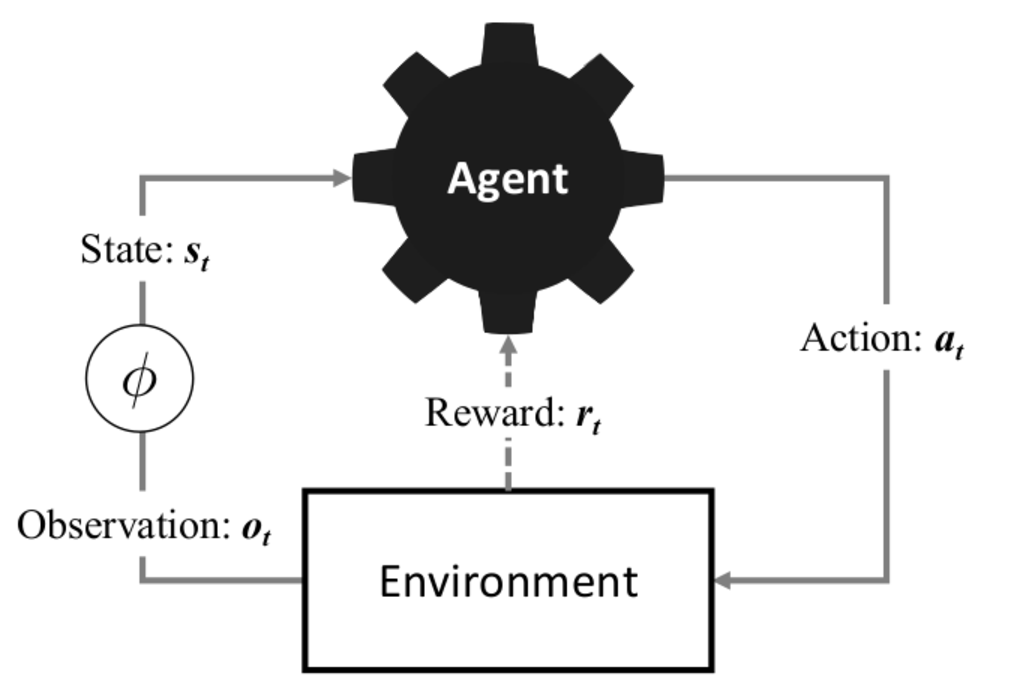
\includegraphics[width=0.6\textwidth]{images/fmlpda_figure_11_1.pdf}
       \caption{An agent behaving in an environment and the observation, reward, action cycle. The transition from observations of the environment to a state is shown by the state generation function, $\phi$.}
       \label{fig:rl_framework}
       \end{centering}
\end{figure}
\end{frame} 



 \begin{frame} 
\begin{equation}
(s_1, a_1, r_1), (s_2, a_2, r_2), (s_3, a_3, r_3), \ldots ,(s_e, a_e, r_e)
\end{equation}
\end{frame} 


\subsection{Fundamentals of Reinforcement Learning}



 \begin{frame} 
 \begin{equation}
G = r_t + r_{t+1}+r_{t+2} +r_{t+3} + \ldots +r_{e}
\label{eqn:rerurn_def}
\end{equation}
\end{frame} 



 \begin{frame} 
\begin{equation}
a_t = \pi(s_t)
\end{equation}

~\\

\begin{equation}
\label{eqn:policy_prob_dist}
P(A_t = a \mid S_t = s) = \pi(S_t = s)
\end{equation}
\end{frame} 



 \begin{frame} 
\begin{equation}
V_{\pi}(s_t) = E_{\pi}[r_t + r_{t+1}+r_{t+2} +r_{t+3} + \ldots +r_{e} \mid s_t]
\label{eqn:value_function}
\end{equation}

~\\

\begin{equation}
Q_{\pi}(s_t, a_t) = E_{\pi}[r_t + r_{t+1}+r_{t+2} +r_{t+3} + \ldots +r_{e} \mid s_t, a_t]
\label{eqn:action_value_function}
\end{equation}
\end{frame} 



 \begin{frame} 
\begin{equation}
G_{\gamma} = r_t + \gamma r_{t+1}+ \gamma^2 r_{t+2} + \gamma^3 r_{t+3} + \ldots + \gamma^{e-t} r_{e}
\label{eqn:discount_return_def}
\end{equation}

~\\

\begin{equation*}
G_{\gamma=0.1} = r_t + 0.1 \times r_{t+1}+  0.01 \times r_{t+2} + 0.001 \times r_{t+3} + \ldots
\end{equation*}

~\\

\begin{equation*}
G_{\gamma=0.9} = r_t + 0.9 \times r_{t+1}+  0.81 \times r_{t+2} + 0.729 \times r_{t+3} + \ldots
\end{equation*}
\end{frame} 



 \begin{frame} 
\begin{equation}
Q_{\pi}(s_t, a_t) = E_{\pi}[r_t + \gamma r_{t+1}+\gamma^2 r_{t+2} +\gamma^3 r_{t+3} + \ldots +\gamma^{3-t} r_{e} \mid s_t, a_t]
\label{eqn:discounted_expected_reward}
\end{equation}
\end{frame} 


\subsection{Markov Decision Processes}

 \begin{frame} 
\begin{figure}[tbh]
\begin{centering}
{\setlength{\tabcolsep}{0.05em}
\begin{tabular}{cc}
     \subfigure[S-I-R Markov process]{\label{fig:markov_process_graph}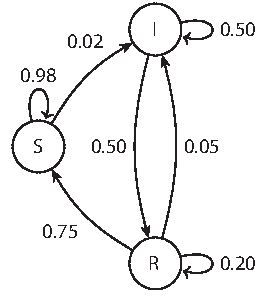
\includegraphics[width=0.4\linewidth]{images/fmlpda_figure_11_2_a.pdf}} & 
     \subfigure[S-I-R transition matrix]{\label{fig:markov_process_matrix}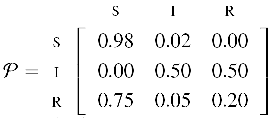
\includegraphics[width=0.5\textwidth]{images/fmlpda_figure_11_2_b.pdf}} \\
\end{tabular}}
\end{centering}
\caption{A simple Markov process to model the evolution of an infectious disease in individuals during an epidemic using the \rlState{Susceptible}-\rlState{Infected}-\rlState{Recovered} (S-I-R) model.}
\label{fig:markov_process}
\end{figure}
\end{frame} 



 \begin{frame} 
\begin{equation}
\label{eqn:markov_assumption_1}
P(S_{t + 1} \mid S_{t}, S_{t-1}, S_{t-2}, \ldots) = P(S_{t + 1} \mid S_{t})
\end{equation}

~\\

\begin{equation}
\label{eqn:markov_assumption_2}
P({s_{1} \rightarrow s_{2}}) = P(S_{t + 1}=s_{2} \mid S_{t}=s_{1})
\end{equation}

~\\

\begin{equation*}
\mathcal{P}  = \begin{bmatrix}
P({s_{1}\rightarrow s_{1}}) & P({s_{1}\rightarrow s_{2}}) & \dots     & P({s_{1}\rightarrow s_{n}}) \\
P({s_{2}\rightarrow s_{1}}) & P({s_{2}\rightarrow s_{2}}) & \dots     & P({s_{2}\rightarrow s_{n}}) \\
\vdots  &  \vdots   &  \ddots   &   \vdots  \\   
P({s_{n}\rightarrow s_{1}}) & P({s_{n}\rightarrow s_{2}}) & \dots     & P({s_{n}\rightarrow s_{n}}) \\
            \end{bmatrix}
\end{equation*}
\end{frame} 



 \begin{frame} 
\begin{equation}
\label{eqn:markov_assumption}
P({s_{1} \xrightarrow[]{a} s_{2}}) = P(S_{t + 1}=s_{2} \mid S_{t}=s_{1}, A_{t}=a)
\end{equation}

~\\

\begin{equation}
\label{eqn:expecrted_reward}
R({s_{1} \xrightarrow[]{a} s_{2}}) = E(r_t \mid S_t = s_1, S_{t+1}=s_2, A_t =a)
\end{equation}
\end{frame} 



 \begin{frame} 
\begin{table}[!t]
\caption{Some episodes of games played by the TwentyTwos agent showing the cards dealt, as well as the states, actions, and rewards. Note that rewards are shown on the row indicating the action that led to them, not the state that followed that action.}
\label{table:blackjack_demo}
\begin{scriptsize}

{\setlength{\tabcolsep}{0.3em}
\begin{tabular*}{\textwidth}{@{\extracolsep{\fill}} rlrlrllr @{}}
\Toprule
Iter & \multicolumn{2}{l}{Player Hand} & \multicolumn{2}{l}{Dealer Hand} & State &  Action & Reward \\
\Midrule
1 & $2\,\varheart$ $7\,\varclub$ &  $(9)$ & $8\,\varheart$ & $(8)$ & \rlState{PL-DH} & \rlAction{Twist} &  0 \\
2 & $2\,\varheart$ $7\,\varclub$ $K\,\varclub$ & $(19)$ & $8\,\varheart$ & $(8)$ & \rlState{PH-DH} & \rlAction{Stick} &  +1 \\
3 & $2\,\varheart$ $7\,\varclub$ $K\,\varclub$ & $(19)$ & $8\,\varheart$ $Q\,\vardiamond$ & $(18)$ & \rlState{Win} & &  ~ \\
\Midrule
1 & $4\,\spadesuit$ $A\,\varheart$ &  $(15)$ & $Q\,\varheart$ & $(10)$ & \rlState{PM-DH} & \rlAction{Twist} &  -1 \\
2 & $4\,\spadesuit$ $A\,\varheart$ $9\,\varclub$ & $(24)$ & $Q\,\varheart$ & $(10)$ & \rlState{Bust} &  & $ ~$ \\
\Midrule
1 & $2\,\vardiamond$ $4\,\vardiamond$ &  $(6)$ & $3\,\varheart$ & $(3)$ & \rlState{PL-DL} & \rlAction{Twist} &  0 \\
2 & $2\,\vardiamond$ $4\,\vardiamond$  $3\,\varheart$&  $(9)$ & $3\,\varheart$ & $(3)$ & \rlState{PL-DL} & \rlAction{Twist} &  0 \\
3 & $2\,\vardiamond$ $4\,\vardiamond$  $3\,\varheart$ $6\,\varclub$ &  $(15)$ & $3\,\varheart$ & $(3)$ & \rlState{PM-DL} & \rlAction{Twist} &  0 \\
4 & $2\,\vardiamond$ $4\,\vardiamond$  $3\,\varheart$ $6\,\varclub$  $6\,\vardiamond$ &  $(21)$ & $3\,\varheart$ & $(3)$ & \rlState{PH-DL} & \rlAction{Stick} &  0 \\
5 & $2\,\vardiamond$ $4\,\vardiamond$  $3\,\varheart$ $6\,\varclub$  $6\,\vardiamond$ &  $(21)$ & $3\,\varheart$ $7\,\varheart$ $A\,\spadesuit$ & $(21)$ & \rlState{Tie} & ~ &  ~ \\
\Midrule
1 & $Q\,\vardiamond$ $J\,\varclub$ &  $(20)$ & $A\,\varheart$ & $(11)$ & \rlState{PH-DH} & \rlAction{Stick} &  +1 \\
2 & $Q\,\vardiamond$ $J\,\varclub$ &  $(20)$ & $A\,\varclub$ $5\,\varclub$ $Q\,\spadesuit$ & $(26)$ & \rlState{Win} &  &  ~ \\
\Midrule
1 & $A\,\vardiamond$ $A\,\varheart$ &  $(22)$ & $2\,\varheart$ & $(2)$ & \rlState{PH-DL} & \rlAction{Stick} &  +2 \\
2 & $A\,\vardiamond$ $A\,\varheart$ &  $(22)$ & $2\,\varheart$ & $(2)$ & \rlState{TwentyTwo} &  &  ~ \\
\Botrule
\end{tabular*}
}
{}
\end{scriptsize}
\end{table}
\end{frame} 



 \begin{frame}[plain]
\begin{figure}[!t]
\begin{centering}
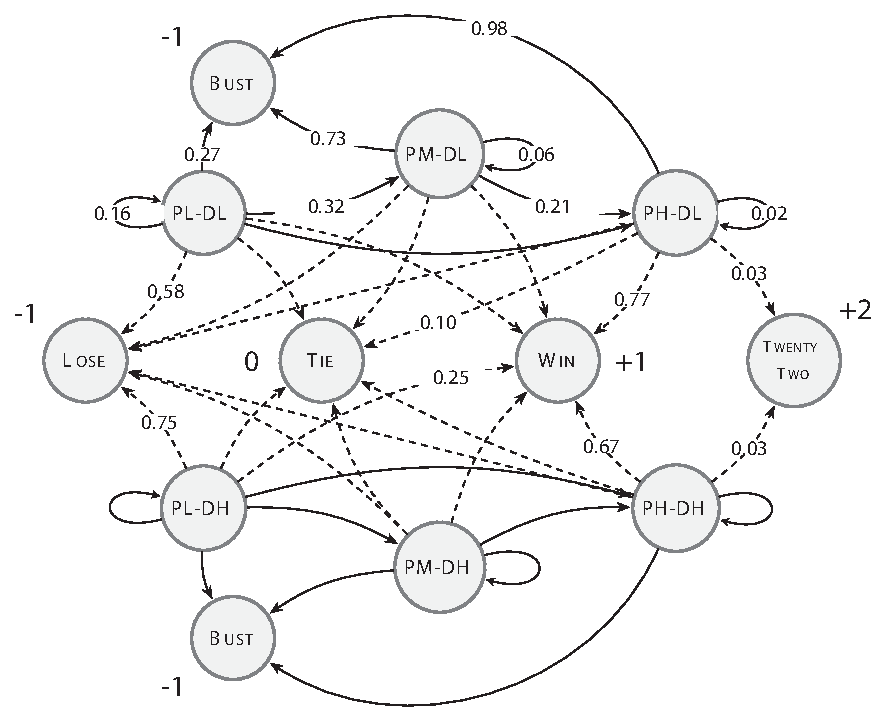
\includegraphics[width=0.9\linewidth]{images/fmlpda_figure_11_3.pdf}
 \caption{A Markov decision process representation for TwentyTwos, a simplified version of the card game Blackjack.}
       \label{fig:blackjack_mdp}
       \end{centering}
\end{figure}
\end{frame} 



 \begin{frame} 
\resizebox{0.9\textwidth}{!}{
 \begin{minipage}{\textwidth}
\begin{equation*}
\begin{tiny}
\mathcal{P}^{ \rlAction{Twist}} = \begin{bmatrix}
P(\rlState{PL-DL} \xrightarrow[]{\rlAction{Twist}} \rlState{PL-DL}) & P(\rlState{PL-DL} \xrightarrow[]{\rlAction{Twist}} \rlState{PM-DL}) & \dots     & P(\rlState{PL-DL} \xrightarrow[]{\rlAction{Twist}} \rlState{TwentyTwo}) \\
P(\rlState{PM-DL} \xrightarrow[]{\rlAction{Twist}} \rlState{PL-DL}) & P(\rlState{PM-DL} \xrightarrow[]{\rlAction{Twist}} \rlState{PM-DL}) & \dots     & P(\rlState{PM-DL} \xrightarrow[]{\rlAction{Twist}} \rlState{TwentyTwo}) \\
\vdots  &  \vdots   &  \ddots   &   \vdots  \\   
P(\rlState{TwentyTwo} \xrightarrow[]{\rlAction{Twist}} \rlState{PL-DL}) & P(\rlState{TwentyTwo} \xrightarrow[]{\rlAction{Twist}} \rlState{PM-DL}) & \dots     & P(\rlState{TwentyTwo} \xrightarrow[]{\rlAction{Twist}} \rlState{TwentyTwo}) \\ \\
            \end{bmatrix}
\end{tiny}
\end{equation*}
 \end{minipage}}

~\\

\resizebox{0.9\textwidth}{!}{
 \begin{minipage}{\textwidth}
\begin{equation*}
\begin{tiny}
\mathcal{P}^{ \rlAction{Stick}} = \begin{bmatrix}
P(\rlState{PL-DL} \xrightarrow[]{\rlAction{Stick}} \rlState{PL-DL}) & P(\rlState{PL-DL} \xrightarrow[]{\rlAction{Stick}} \rlState{PM-DL}) & \dots     & P(\rlState{PL-DL} \xrightarrow[]{\rlAction{Stick}} \rlState{TwentyTwo}) \\
P(\rlState{PM-DL} \xrightarrow[]{\rlAction{Stick}} \rlState{PL-DL}) & P(\rlState{PM-DL} \xrightarrow[]{\rlAction{Stick}} \rlState{PM-DL}) & \dots     & P(\rlState{PM-DL} \xrightarrow[]{\rlAction{Stick}} \rlState{TwentyTwo}) \\
\vdots  &  \vdots   &  \ddots   &   \vdots  \\   
P(\rlState{TwentyTwo} \xrightarrow[]{\rlAction{Stick}} \rlState{PL-DL}) & P(\rlState{TwentyTwo} \xrightarrow[]{\rlAction{Stick}} \rlState{PM-DL}) & \dots     & P(\rlState{TwentyTwo} \xrightarrow[]{\rlAction{Stick}} \rlState{TwentyTwo}) \\ \\
            \end{bmatrix}
\end{tiny}
\end{equation*}
 \end{minipage}}
\end{frame} 

\begin{frame}
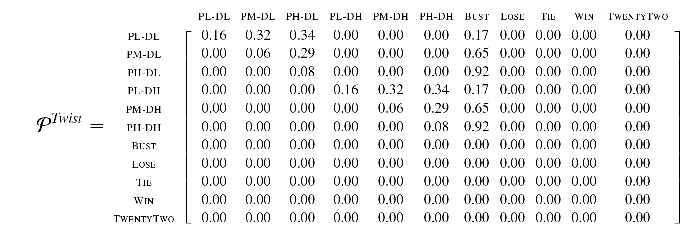
\includegraphics[width=\textwidth]{images/fmlpda_eqn_11_14.pdf}
\end{frame}

\begin{frame}

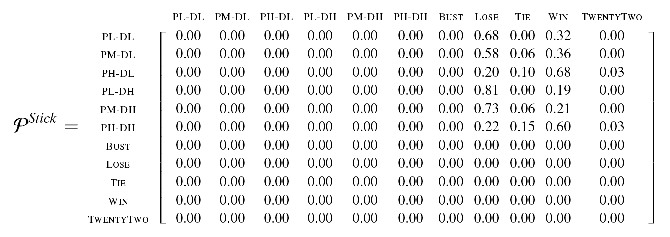
\includegraphics[width=\textwidth]{images/fmlpda_eqn_11_15.pdf}

\end{frame}

% \begin{frame} 
%\begin{equation}
%\label{eqn:transitionMatrixTwist}
%\begin{scriptsize}
%\setlength{\arraycolsep}{2.5pt} % tighten up matrix to save horizontal space.
%\mathcal{P}^{ \rlAction{Twist}}  = 
%    \kbordermatrix{ & \rlState{PL-DL} & \rlState{PM-DL} & \rlState{PH-DL} & \rlState{PL-DH} & \rlState{PM-DH} & \rlState{PH-DH} & \rlState{Bust} & \rlState{Lose} & \rlState{Tie} & \rlState{Win}  & \rlState{TwentyTwo}\\
%      \rlState{PL-DL} & 0.16 & 0.32 & 0.34 & 0.00 & 0.00 & 0.00 & 0.17 & 0.00 & 0.00 & 0.00 & 0.00 \\
%      \rlState{PM-DL} & 0.00 & 0.06 & 0.29 & 0.00 & 0.00 & 0.00 & 0.65 & 0.00 & 0.00 & 0.00 & 0.00 \\
%      \rlState{PH-DL} & 0.00 & 0.00 & 0.08 & 0.00 & 0.00 & 0.00 & 0.92 & 0.00 & 0.00 & 0.00 & 0.00 \\
%      \rlState{PL-DH} & 0.00 & 0.00 & 0.00 & 0.16 & 0.32 & 0.34 & 0.17 & 0.00 & 0.00 & 0.00 & 0.00 \\
%      \rlState{PM-DH} & 0.00 & 0.00 & 0.00 & 0.00 & 0.06 & 0.29 & 0.65 & 0.00 & 0.00 & 0.00 & 0.00 \\
%      \rlState{PH-DH} & 0.00 & 0.00 & 0.00 & 0.00 & 0.00 & 0.08 & 0.92 & 0.00 & 0.00 & 0.00 & 0.00 \\
%      \rlState{Bust} & 0.00 & 0.00 & 0.00 & 0.00 & 0.00 & 0.00 & 0.00 & 0.00 & 0.00 & 0.00 & 0.00 \\
%      \rlState{Lose} & 0.00 & 0.00 & 0.00 & 0.00 & 0.00 & 0.00 & 0.00 & 0.00 & 0.00 & 0.00 & 0.00 \\
%      \rlState{Tie} & 0.00 & 0.00 & 0.00 & 0.00 & 0.00 & 0.00 & 0.00 & 0.00 & 0.00 & 0.00 & 0.00 \\
%      \rlState{Win} & 0.00 & 0.00 & 0.00 & 0.00 & 0.00 & 0.00 & 0.00 & 0.00 & 0.00 & 0.00 & 0.00 \\
%      \rlState{TwentyTwo} & 0.00 & 0.00 & 0.00 & 0.00 & 0.00 & 0.00 & 0.00 & 0.00 & 0.00 & 0.00 & 0.00} \\
%\end{scriptsize}
%\end{equation}
%\end{frame} 



% \begin{frame} 
%\begin{equation}
%\label{eqn:transitionMatrixStick}
%\begin{scriptsize}
%\setlength{\arraycolsep}{2.5pt} % tighten up matrix to save horizontal space.
%\mathcal{P}^{ \rlAction{Stick}}  =  
%    \kbordermatrix{ & \rlState{PL-DL} & \rlState{PM-DL} & \rlState{PH-DL} & \rlState{PL-DH} & \rlState{PM-DH} & \rlState{PH-DH} & \rlState{Bust} & \rlState{Lose} & \rlState{Tie} & \rlState{Win}  & \rlState{TwentyTwo}\\
%      \rlState{PL-DL} & 0.00 &    0.00 &    0.00 &    0.00 &    0.00 &    0.00 &   0.00 &  0.68 &  0.00 &  0.32 &      0.00 \\
%      \rlState{PM-DL} & 0.00 &    0.00 &    0.00 &    0.00 &    0.00 &    0.00 &   0.00 &  0.58 &  0.06 &  0.36 &      0.00 \\
%      \rlState{PH-DL} & 0.00 &    0.00 &    0.00 &    0.00 &    0.00 &    0.00 &   0.00 &  0.20 &  0.10 &  0.68 &      0.03 \\
%      \rlState{PL-DH} & 0.00 &    0.00 &    0.00 &    0.00 &    0.00 &    0.00 &   0.00 &  0.81 &  0.00 &  0.19 &      0.00 \\
%      \rlState{PM-DH} & 0.00 &    0.00 &    0.00 &    0.00 &    0.00 &    0.00 &   0.00 &  0.73 &  0.06 &  0.21 &      0.00 \\
%      \rlState{PH-DH} & 0.00 &    0.00 &    0.00 &    0.00 &    0.00 &    0.00 &   0.00 &  0.22 &  0.15 &  0.60 &      0.03 \\
%      \rlState{Bust} & 0.00 & 0.00 & 0.00 & 0.00 & 0.00 & 0.00 & 0.00 & 0.00 & 0.00 & 0.00 & 0.00 \\
%      \rlState{Lose} & 0.00 & 0.00 & 0.00 & 0.00 & 0.00 & 0.00 & 0.00 & 0.00 & 0.00 & 0.00 & 0.00 \\
%      \rlState{Tie} & 0.00 & 0.00 & 0.00 & 0.00 & 0.00 & 0.00 & 0.00 & 0.00 & 0.00 & 0.00 & 0.00 \\
%      \rlState{Win} & 0.00 & 0.00 & 0.00 & 0.00 & 0.00 & 0.00 & 0.00 & 0.00 & 0.00 & 0.00 & 0.00 \\
%      \rlState{TwentyTwo} & 0.00 & 0.00 & 0.00 & 0.00 & 0.00 & 0.00 & 0.00 & 0.00 & 0.00 & 0.00 & 0.00} \\
%\end{scriptsize}
%\end{equation}
%\end{frame} 


\subsection{The Bellman Equations}



 \begin{frame} 
\begin{eqnarray}
\label{eqn:bellman_step1}
Q_{\pi}(s_t, a_t) &= & E_{\pi}\left[r_t + \gamma r_{t+1}+\gamma^2 r_{t+2}  + \ldots +\gamma^3 r_{\infty} \mid s_t, a_t\right] \nonumber \\
			\label{eqn:bellman_step2}
			 & = & E_{\pi}\left[\sum_{k=0}^{\infty}\gamma^{k} r_{t+k}\mid s_t, a_t\right]  \\
			 \label{eqn:bellman_step3}
			 & = & E_{\pi}\left[r_t + \gamma\sum_{k=0}^{\infty}\gamma^{k} r_{t+k+1} \mid s_t, a_t\right] 
\end{eqnarray} 
\end{frame} 



 \begin{frame} 
 \resizebox{0.8\textwidth}{!}{
 \begin{minipage}{\textwidth}
\begin{equation}
			 \label{eqn:bellman_step4}
Q_{\pi}(s_t, a_t)  =  \sum_{s_{t+1}}  P({s_{t}\xrightarrow[]{a_t}s_{t+1}})  \left[R({s_{t} \xrightarrow[]{a_t} s_{t+1}}) + \gamma E_{\pi}\left[\sum_{k=0}^{\infty}\gamma^{k} r_{t+k+1} \mid s_{t+1}\right]\right] 
\end{equation} 
 \end{minipage}}

~\\

  \resizebox{0.74\textwidth}{!}{
 \begin{minipage}{\textwidth}
\begin{eqnarray}
			\label{eqn:bellman_step5}
Q_{\pi}(s_t, a_t) =  \sum_{s_{t+1}}  P({s_{t}\xrightarrow[]{a_t} s_{t+1}})  \left[R({s_{t} \xrightarrow[]{a_t} s_{t+1}}) + \gamma \sum_{a_{t+1}}E_{\pi}\left[\sum_{k=0}^{\infty}\gamma^{k} r_{t+k+1} \mid s_{t+1}, a_{t+1}\right]\right] \nonumber \\
~ 
\end{eqnarray}
  \end{minipage}}

~\\

  \resizebox{0.74\textwidth}{!}{
 \begin{minipage}{\textwidth}
\begin{eqnarray}
			\label{eqn:bellman_step6}
Q_{\pi}(s_t, a_t) =   \sum_{s_{t+1}}  P({s_{t}\xrightarrow[]{a_t} s_{t+1}})  \left[R({s_{t} \xrightarrow[]{a_t} s_{t+1}}) + \gamma\sum_{a_{t+1}} \pi(s_{t+1}, a_{t+1})Q_{\pi}(s_{t+1}, a_{t+1})\right]   \nonumber \\
			%Maybe could replace two lines above with these two lines as we are assuming a single action is returned - passive policy. 
			%& = & \sum_{s_{t+1}}  P({s_{t}\xrightarrow[]{a_t} s_{t+1}})  \left[R({s_{t} \xrightarrow[]{a_t} s_{t+1}}) + \gamma Q_{\pi}(s_{t+1}, \pi(s_{t+1}))\right] \\
~
\end{eqnarray}
  \end{minipage}}

~\\

  \resizebox{0.74\textwidth}{!}{
 \begin{minipage}{\textwidth}
\begin{equation}
Q_{*}(s_t, a_t) =  \sum_{s_{t+1}}  P({s_{t}\xrightarrow[]{a_t}s_{t+1}})  \left[R({s_{t} \xrightarrow[]{a_t} s_{t+1}}) + \gamma \max_{a_{t+1}}Q_{*}(s_{t+1}, a_{t+1})\right] 
			\label{eqn:bellman_optimality}
\end{equation}
  \end{minipage}}
\end{frame} 


\subsection{Temporal-Difference Learning}



 \begin{frame} 
\begin{table}[htb]
\caption{An action-value table for an agent trained to play the card game TwentyTwos (the simplified version of Blackjack described in Section \ourRef{sec:rl_mdps}).}
\label{tab:bj_action_value_table_intial}
\begin{scriptsize}
{\setlength{\tabcolsep}{0.4em}
\begin{tabular*}{25pc}{llr}
\Toprule
\begin{minipage}{0.28\textwidth}
\raggedright
{\setlength{\tabcolsep}{0.1em}
\begin{tabular*}{7pc}{@{\extracolsep{\fill}} llr @{}}
State & Action & Value \\
\Midrule
\rlState{PL-DL} & \rlAction{Twist} & $0.039$ \\
\rlState{PL-DL} & \rlAction{Stick} & $-0.623$ \\
\rlState{PM-DL} & \rlAction{Twist} & $-0.597$ \\
\rlState{PM-DL} & \rlAction{Stick} & $-0.574$ \\
\rlState{Bust} & \rlAction{Twist} & $0.000$ \\ 
\rlState{Bust} & \rlAction{Stick} & $0.000$ \\ 
\rlState{Lose} & \rlAction{Twist} & $0.000$ \\ 
\rlState{Lose} & \rlAction{Stick} & $0.000$ \\ 
\Botrule
\end{tabular*}
}
\end{minipage}
&
\begin{minipage}{0.28\textwidth}
\centering
{\setlength{\tabcolsep}{0.1em}
\begin{tabular*}{7pc}{@{\extracolsep{\fill}} l l r @{}}
State & Action & Value \\
\Midrule
\rlState{PH-DL} & \rlAction{Twist} & $-0.666$ \\
\rlState{PH-DL} & \rlAction{Stick} & $0.940$ \\
\rlState{PL-DH} & \rlAction{Twist} & $-0.159$ \\
\rlState{PL-DH} & \rlAction{Stick} & $-0.379$ \\
\rlState{Tie} & \rlAction{Twist} & $0.000$ \\ 
\rlState{Tie} & \rlAction{Stick} & $0.000$ \\ 
~ & ~ & ~ \\ 
~ & ~ & ~ \\ 
\Botrule
\end{tabular*}
}
\end{minipage}
&
\begin{minipage}{0.28\textwidth}
\raggedleft
{\setlength{\tabcolsep}{0.7em}
\begin{tabular*}{10pc}{@{\extracolsep{\fill}} l l r @{}}
State & Action & Value \\
\Midrule
\rlState{PM-DH} & \rlAction{Twist} & $-0.668$ \\
\rlState{PM-DH} & \rlAction{Stick} & $-0.852$ \\
\rlState{PH-DH} & \rlAction{Twist} & $-0.883$ \\
\rlState{PH-DH} & \rlAction{Stick} & $0.391$ \\
\rlState{Win} & \rlAction{Twist} & $0.000$ \\ 
\rlState{Win} & \rlAction{Stick} & $0.000$ \\  
\rlState{TwentyTwo} & \rlAction{Twist} & $0.000$ \\ 
\rlState{TwentyTwo} & \rlAction{Stick} & $0.000$ \\  
\Botrule
\end{tabular*}
}
\end{minipage}\\
\end{tabular*}
}{}
\end{scriptsize}
\end{table}
\end{frame} 



 \begin{frame} 
\begin{equation}
Q_{\pi}\left(s_t, a_t\right) \leftarrow Q_{\pi}\left(s_t, a_t\right) + \alpha(\underbrace{G\left(s_t, a_t\right) - Q_{\pi}\left(s_t, a_t\right)}_{\substack{
		\text{difference between actual}\\
		\text{and expected returns}
	}})
\label{eqn:td_learning_basic}
\end{equation}
\end{frame} 



 \begin{frame} 
\begin{equation}
Q_{\pi}\left(s_t, a_t\right) \leftarrow Q_{\pi}\left(s_t, a_t\right) + \alpha(\underbrace{r_t + \gamma  Q_{\pi}\left(s_{t+1}, a_{t+1}\right)}_{
	\substack{
		\text{actual}\\
		\text{return}
	}} - \underbrace{Q_{\pi}\left(s_t, a_t\right)}_{\substack{
		\text{expected}\\
		\text{return}
	}})
\label{eqn:td_learning}
\end{equation}
\end{frame} 


\SectionSlide{Standard Approach: Q-Learning, Off-Policy Temporal-Difference Learning}



 \begin{frame} 
 \begin{footnotesize}
    \begin{equation}
    {Q}\left({s_t}, {a_t}\right) \leftarrow {Q}\left({s_t}, {a_t}\right) + \alpha\left({r_t} + \gamma\max_{{a_{t+1}}}{Q}\left({s_{t+1}}, a_{t+1}\right) - {Q}\left({s_t}, {a_t}\right)\right)
    \label{eqn:q_learning_alg}
     \end{equation}
     \end{footnotesize}
\end{frame} 

\begin{frame}[plain]
\scriptsize{Pseudocode description of the Q-learning algorithm for off-policy temporal-difference learning.}

\begin{footnotesize}
%\begin{algorithm}[htb]
%\caption{Pseudocode description of the Q-learning algorithm for off-policy temporal-difference learning.}
%\label{alg:q_learning}
\begin{algorithmic}[1]
\Require a behavior policy, $\pi$, that chooses actions
\Require an action-value function $Q$ that performs a lookup into an action-value table with entries for every possible action, $a$, and state, $s$
\Require a learning rate, $\alpha$, a discount-rate, $\gamma$, and a number of episodes to perform
\State initialize all entries in the action-value table to random values (except for terminal states which receive a value of $0$)
\label{alg_ln:ql_intialise_q_table}
\For{each episode}
\State reset $s_{t}$ to the initial agent state
\label{alg_ln:ql_intialise_agent_state}
\Repeat
    \State{select an action, ${a_t}$, based on policy, $\pi$, current state, ${s_t}$, and action-value function, ${Q}$ }
    \label{alg_ln:ql_choose_action}
    \State take action ${a_t}$ observing reward, ${r_t}$, and new state ${s_{t+1}}$
     \label{alg_ln:ql_take_action}
    \State{update the record in the action-value table for the action, $a_t$, just taken in the last state, $s_t$, using: 
     \label{alg_ln:ql_update_q_value}
    \begin{equation}
    {Q}\left({s_t}, {a_t}\right) \leftarrow {Q}\left({s_t}, {a_t}\right) + \alpha\left({r_t} + \gamma\max_{{a_{t+1}}}{Q}\left({s_{t+1}}, a_{t+1}\right) - {Q}\left({s_t}, {a_t}\right)\right)
    \label{eqn:q_learning_alg}
     \end{equation}}
     \State let $s_t = s_{t+1}$
      \label{alg_ln:ql_update_state}
\Until{agent reaches a terminal state}
\EndFor
\end{algorithmic}
%\end{algorithm}
\end{footnotesize}
\end{frame}

\subsection{A Worked Example}



 \begin{frame} 
\begin{figure}[htb]
       \begin{centering}
       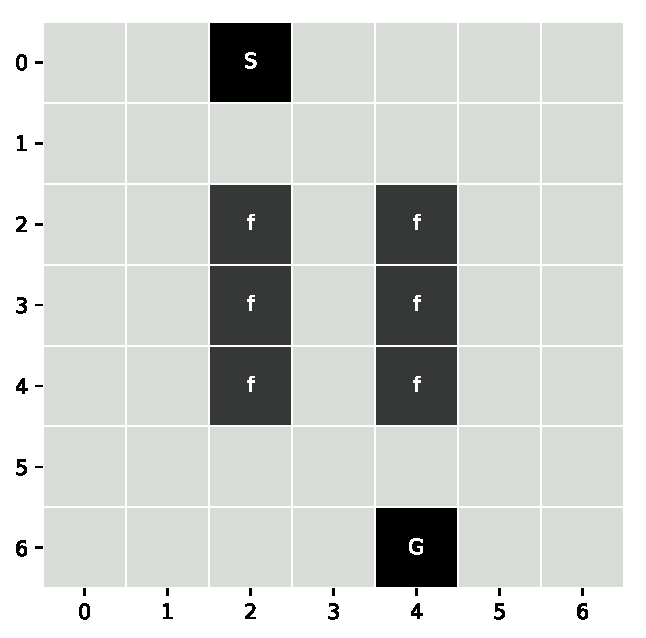
\includegraphics[width=0.45\textwidth]{images/fmlpda_figure_11_4.pdf}
       \caption{A simple grid world. The start position is annotated with an \textit{S} and the goal with a \textit{G}. The squares marked \textit{f} denote fire, which is very damaging to an agent.}
       \label{fig:rl_grid_world}
       \end{centering}
\end{figure}
\end{frame} 



 \begin{frame}[plain]
\begin{table}[tb]
\caption{A portion of the action-value table for the grid world example at its first initialization.}
\label{tab:gridworld_intial_table}
\begin{footnotesize}
{\setlength{\tabcolsep}{0em}
\begin{tabular*}{0.985\linewidth}{llr}
\Toprule
\begin{minipage}{0.33\textwidth}
\raggedright
{\setlength{\tabcolsep}{0.1em}
\begin{tabular*}{7pc}{@{\extracolsep{\fill}} llr @{}}
State & Action & Value \\
\Midrule
\rlState{0-0} & \rlAction{up} & $0.933$ \\ 
\rlState{0-0} & \rlAction{down} & $-0.119$ \\ 
\rlState{0-0} & \rlAction{left} & $-0.985$ \\ 
\rlState{0-0} & \rlAction{right} & $0.822$ \\ 
\rlState{0-1} & \rlAction{up} & $0.879$ \\ 
\rlState{0-1} & \rlAction{down} & $0.164$ \\ 
\rlState{0-1} & \rlAction{left} & $0.343$ \\ 
\rlState{0-1} & \rlAction{right} & $-0.832$ \\ 
\rlState{0-2} & \rlAction{up} & $0.223$ \\ 
\rlState{0-2} & \rlAction{down} & $0.582$ \\ 
\rlState{0-2} & \rlAction{left} & $0.672$ \\ 
\rlState{0-2} & \rlAction{right} & $0.084$ \\ 
\rlState{0-3} & \rlAction{up} & $-0.308$ \\ 
\rlState{0-3} & \rlAction{down} & $0.247$ \\ 
\rlState{0-3} & \rlAction{left} & $0.963$ \\ 
\rlState{0-3} & \rlAction{right} & $0.455$ \\ 
\rlState{0-4} & \rlAction{up} & $-0.634$ \\ 
\multicolumn{3}{c}{$\ldots$} \\
\Botrule
\end{tabular*}
}
			\end{minipage}
			&
			\begin{minipage}{0.33\textwidth}
			\centering
			{\setlength{\tabcolsep}{0.1em}
					%\begin{tabular}[ht]{ c r r }
					\begin{tabular*}{7pc}{@{\extracolsep{\fill}} l l r @{}}
State & Action & Value \\
\Midrule
\multicolumn{3}{c}{$\ldots$} \\
\rlState{2-0} & \rlAction{left} & $-0.691$ \\ 
\rlState{2-0} & \rlAction{right} & $0.668$ \\ 
\rlState{2-1} & \rlAction{up} & $-0.918$ \\ 
\rlState{2-1} & \rlAction{down} & $-0.228$ \\ 
\rlState{2-1} & \rlAction{left} & $-0.301$ \\ 
\rlState{2-1} & \rlAction{right} & $-0.317$ \\ 
\rlState{2-2} & \rlAction{up} & $0.633$ \\ 
\rlState{2-2} & \rlAction{down} & $-0.048$ \\ 
\rlState{2-2} & \rlAction{left} & $0.566$ \\ 
\rlState{2-2} & \rlAction{right} & $-0.058$ \\ 
\rlState{2-3} & \rlAction{up} & $0.635$ \\ 
\rlState{2-3} & \rlAction{down} & $0.763$ \\ 
\rlState{2-3} & \rlAction{left} & $-0.121$ \\ 
\rlState{2-3} & \rlAction{right} & $0.562$ \\ 
\rlState{2-4} & \rlAction{up} & $0.629$ \\ 
\rlState{2-4} & \rlAction{down} & $-0.409$ \\ 
\multicolumn{3}{c}{$\ldots$} \\
\Botrule
				\end{tabular*}
}
			\end{minipage}
			&
			\begin{minipage}{0.33\textwidth}
			\raggedleft
{\setlength{\tabcolsep}{0.7em}
\begin{tabular*}{7pc}{@{\extracolsep{\fill}} l l r @{}}
State & Action & Value \\
\Midrule
\multicolumn{3}{c}{$\ldots$} \\
\rlState{6-2} & \rlAction{right} & $0.201$ \\ 
\rlState{6-3} & \rlAction{up} & $-0.588$ \\ 
\rlState{6-3} & \rlAction{down} & $0.038$ \\ 
\rlState{6-3} & \rlAction{left} & $0.859$ \\ 
\rlState{6-3} & \rlAction{right} & $-0.085$ \\ 
\rlState{6-4} & \rlAction{up} & $0.000$ \\ 
\rlState{6-4} & \rlAction{down} & $0.000$ \\ 
\rlState{6-4} & \rlAction{left} & $0.000$ \\ 
\rlState{6-4} & \rlAction{right} & $0.000$ \\ 
\rlState{6-5} & \rlAction{up} & $0.321$ \\ 
\rlState{6-5} & \rlAction{down} & $-0.793$ \\ 
\rlState{6-5} & \rlAction{left} & $-0.267$ \\ 
\rlState{6-5} & \rlAction{right} & $0.588$ \\ 
\rlState{6-6} & \rlAction{up} & $-0.870$ \\ 
\rlState{6-6} & \rlAction{down} & $-0.720$ \\ 
\rlState{6-6} & \rlAction{left} & $0.811$ \\ 
\rlState{6-6} & \rlAction{right} & $0.176$ \\  
\Botrule
\end{tabular*}
}
\end{minipage}\\
\end{tabular*}
}{}
\end{footnotesize}
\end{table}
\end{frame} 



 \begin{frame} 
 \resizebox{\textwidth}{!}{
 \begin{minipage}{\textwidth}
\begin{alignat*}{2}
    {Q}\left(\rlState{0-3}, \rlAction{left}\right) \leftarrow & {Q}\left(\rlState{0-3}, \rlAction{left}\right) + \alpha\times\left({R}\left(\rlState{0-3}, \rlAction{left}\right) + \gamma\times Q(\rlState{0-2},\rlAction{left}) - {Q}\left(\rlState{0-3}, \rlAction{left}\right)\right) \\
    ~ &  0.963 + 0.2\times\left({-1} + 0.9\times 0.672 - 0.963\right) \\
    ~ &  0.691
\end{alignat*}
 \end{minipage}}
\end{frame} 



 \begin{frame} 
  \resizebox{\textwidth}{!}{
 \begin{minipage}{\textwidth}
\begin{alignat*}{2}
    {Q}\left(\rlState{6-5}, \rlAction{left}\right) \leftarrow & {Q}\left(\rlState{6-5}, \rlAction{left}\right) + \alpha\times\left({R}\left(\rlState{6-5}, \rlAction{left}\right) + \gamma\times Q(\rlState{6-4},\rlAction{up}) - {Q}\left(\rlState{6-5}, \rlAction{left}\right)\right) \\
    ~ &  {-0.267} + 0.2\times\left({50} + 0.9\times 0 - {-0.267}\right) \\
    ~ &  9.786
\end{alignat*}
 \end{minipage}}
\end{frame} 



 \begin{frame} 
\begin{figure}[!b]
\begin{center}
{\setlength{\tabcolsep}{0.05em}
\begin{tabular}{r}
	\subfigure[Action-value table after 1 episode]{\label{fig:rl_grid_world_q_learning_ep_0}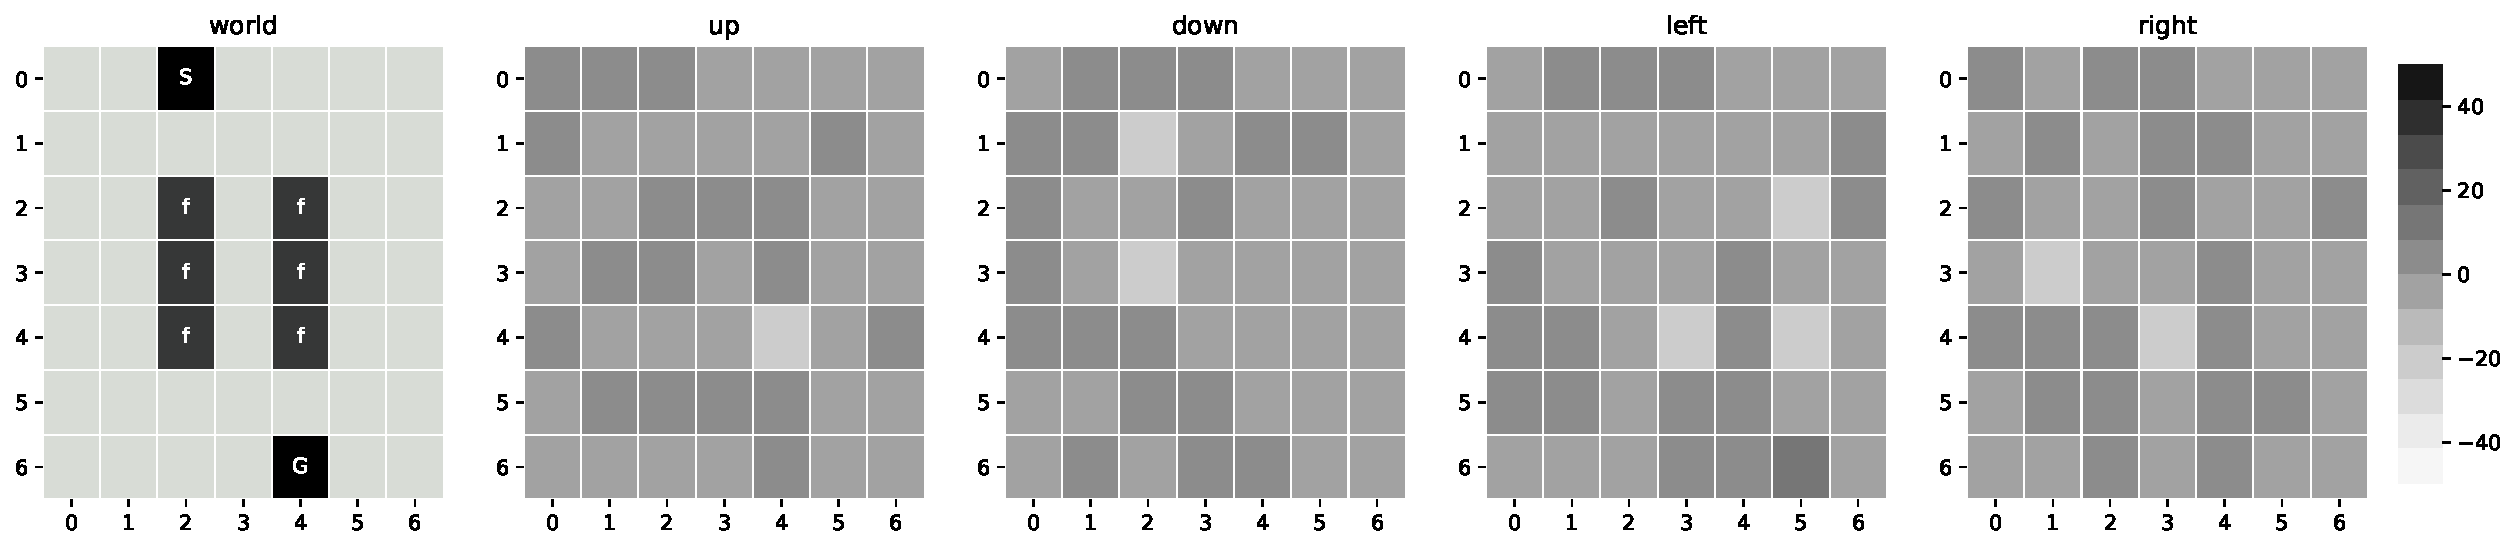
\includegraphics[width=0.98\linewidth]{./images/fmlpda_figure_11_5_a.pdf}} \\
\end{tabular}
}	
\end{center}
\caption[(a)--(c) The evolution of the entries in the action-value table over episodes of Q-learning off-policy temporal-difference learning across the grid world. (d) The cumulative reward earned from each episode.  (e) An illustration of the target policy learned by the agent after $350$ episodes. (f) The path the agent will take from the start state to the goal state when greedily following the target policy.]{(a)--(c) The evolution of the entries in the action-value table over episodes of Q-learning off-policy temporal-difference learning across the grid world. (d) The cumulative reward earned from each episode.  (e) An illustration of the target policy learned by the agent after $350$ episodes. The arrows show the direction with the highest entry in the action-value table for each state. (f) The path the agent will take from the start state to the goal state when greedily following the target policy.}
\label{fig:rl_grid_world_q_learning}
\end{figure}
\end{frame} 


 \begin{frame} 
  \addtocounter{subfigure}{1}
\begin{figure}[!b]
\begin{center}
{\setlength{\tabcolsep}{0.05em}
\begin{tabular}{r}
	\subfigure[Action-value table after 35 episodes]{\label{fig:rl_grid_world_q_learning_ep_30}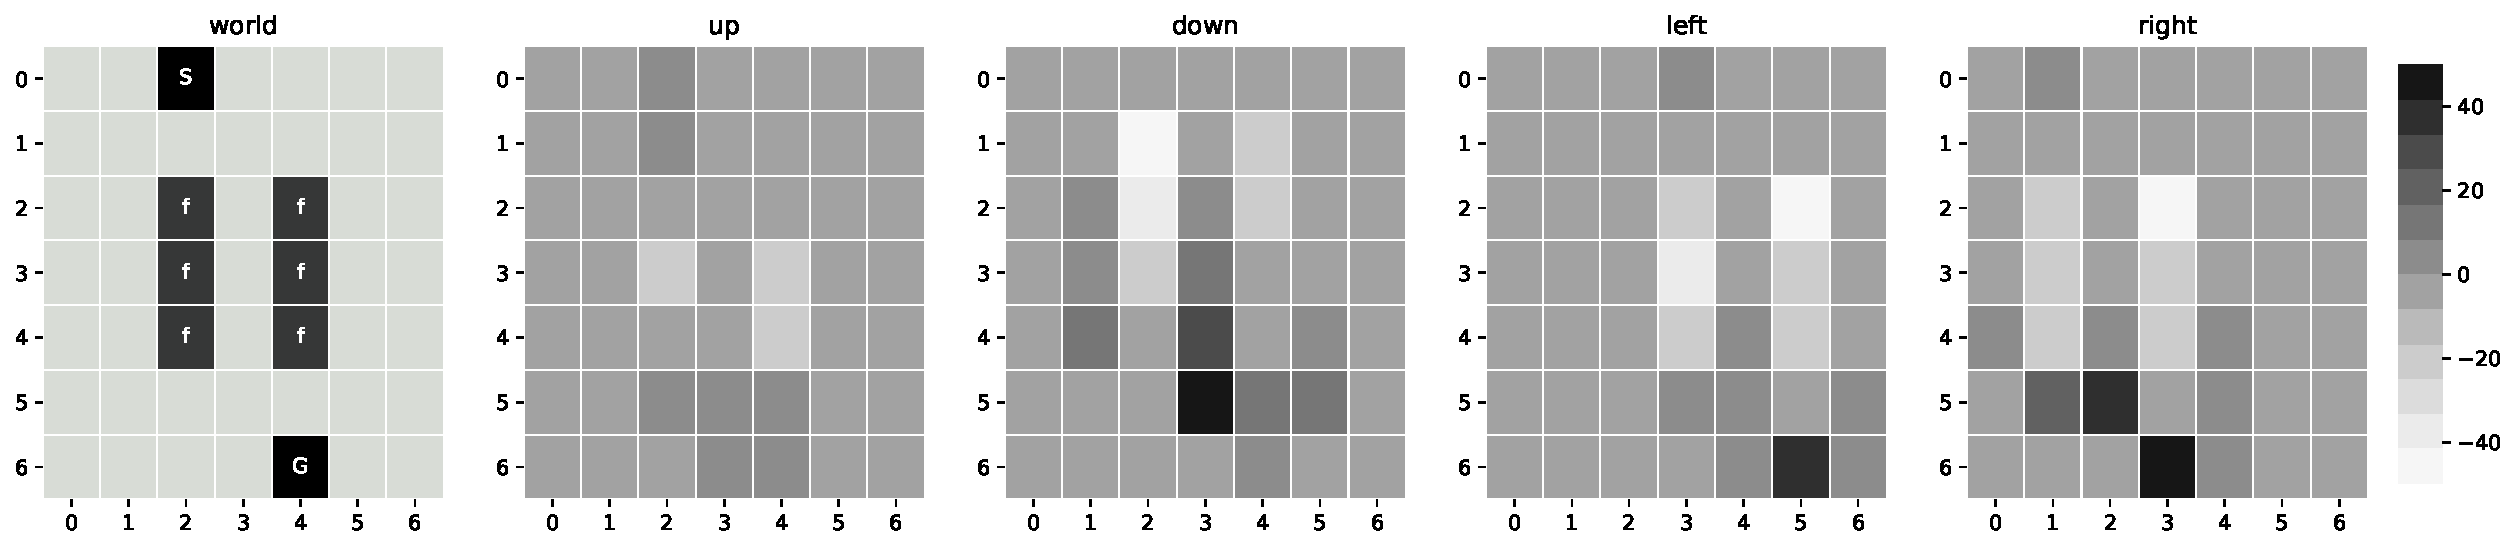
\includegraphics[width=0.98\linewidth]{./images/fmlpda_figure_11_5_b.pdf}} \\
\end{tabular}
}	
\end{center}
\caption[(a)--(c) The evolution of the entries in the action-value table over episodes of Q-learning off-policy temporal-difference learning across the grid world. (d) The cumulative reward earned from each episode.  (e) An illustration of the target policy learned by the agent after $350$ episodes. (f) The path the agent will take from the start state to the goal state when greedily following the target policy.]{(a)--(c) The evolution of the entries in the action-value table over episodes of Q-learning off-policy temporal-difference learning across the grid world. (d) The cumulative reward earned from each episode.  (e) An illustration of the target policy learned by the agent after $350$ episodes. The arrows show the direction with the highest entry in the action-value table for each state. (f) The path the agent will take from the start state to the goal state when greedily following the target policy.}
\label{fig:rl_grid_world_q_learning}
\end{figure}
\end{frame} 


 \begin{frame} 
   \addtocounter{subfigure}{2}
\begin{figure}[!b]
\begin{center}
{\setlength{\tabcolsep}{0.05em}
\begin{tabular}{r}
	\subfigure[Action-value table after 350 episodes]{\label{fig:rl_grid_world_q_learning_ep_100}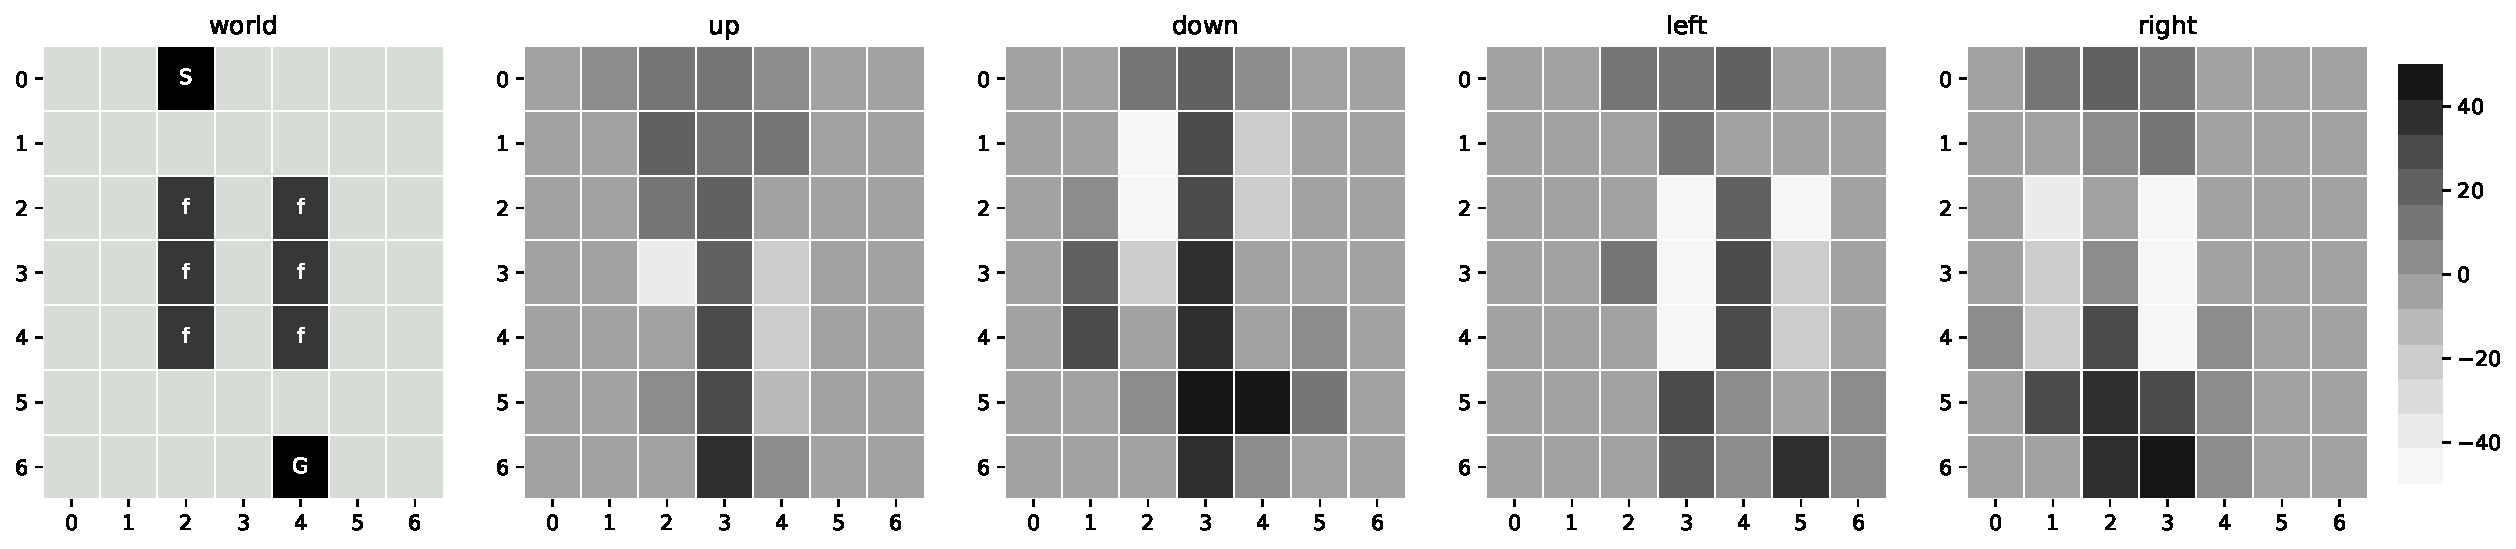
\includegraphics[width=0.98\linewidth]{./images/fmlpda_figure_11_5_c.pdf}} \\
\end{tabular}
}	
\end{center}
\caption[(a)--(c) The evolution of the entries in the action-value table over episodes of Q-learning off-policy temporal-difference learning across the grid world. (d) The cumulative reward earned from each episode.  (e) An illustration of the target policy learned by the agent after $350$ episodes. (f) The path the agent will take from the start state to the goal state when greedily following the target policy.]{(a)--(c) The evolution of the entries in the action-value table over episodes of Q-learning off-policy temporal-difference learning across the grid world. (d) The cumulative reward earned from each episode.  (e) An illustration of the target policy learned by the agent after $350$ episodes. The arrows show the direction with the highest entry in the action-value table for each state. (f) The path the agent will take from the start state to the goal state when greedily following the target policy.}
\label{fig:rl_grid_world_q_learning}
\end{figure}
\end{frame} 


 \begin{frame} 
    \addtocounter{subfigure}{3}
\begin{figure}[!b]
\begin{center}
{\setlength{\tabcolsep}{0.05em}
\begin{tabular}{r}
	\subfigure[Cumulative Reward]{\label{fig:rl_grid_world_q_learning_returns}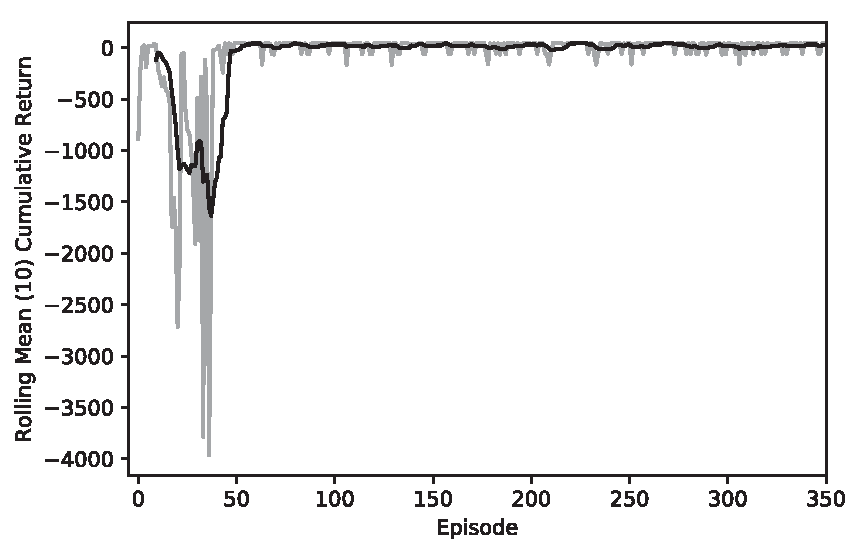
\includegraphics[width=0.37\linewidth]{./images/fmlpda_figure_11_5_d.pdf}} ~\subfigure[Policy]{\label{fig:rl_grid_world_q_learning_policy}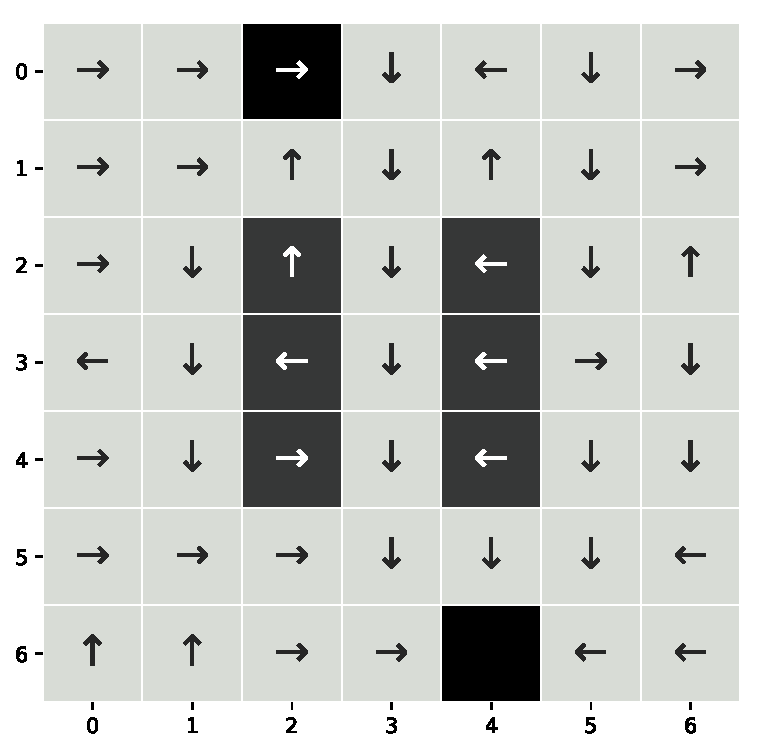
\includegraphics[width=0.24\linewidth]{./images/fmlpda_figure_11_5_e.pdf}}~ \subfigure[Offline Path]{\label{fig:rl_grid_world_q_learning_offline_path}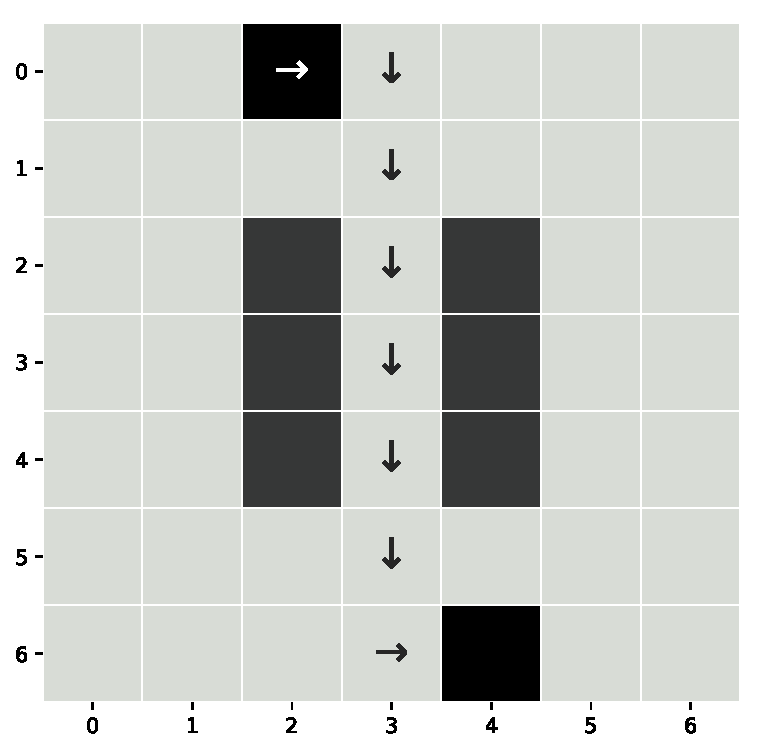
\includegraphics[width=0.24\linewidth]{./images/fmlpda_figure_11_5_f.pdf}}\\
\end{tabular}
}	
\end{center}
\caption[(a)--(c) The evolution of the entries in the action-value table over episodes of Q-learning off-policy temporal-difference learning across the grid world. (d) The cumulative reward earned from each episode.  (e) An illustration of the target policy learned by the agent after $350$ episodes. (f) The path the agent will take from the start state to the goal state when greedily following the target policy.]{(a)--(c) The evolution of the entries in the action-value table over episodes of Q-learning off-policy temporal-difference learning across the grid world. (d) The cumulative reward earned from each episode.  (e) An illustration of the target policy learned by the agent after $350$ episodes. The arrows show the direction with the highest entry in the action-value table for each state. (f) The path the agent will take from the start state to the goal state when greedily following the target policy.}
\label{fig:rl_grid_world_q_learning}
\end{figure}
\end{frame} 

 \begin{frame}[plain]
 \begin{table}[!t]
\caption{A portion of the action-value table for the grid world example after $350$ episodes of Q-learning have elapsed.}
\label{tab:gridworld_final_table}
\begin{footnotesize}
{\setlength{\tabcolsep}{0em}
\begin{tabular*}{0.985\linewidth}{llr}
\Toprule
\begin{minipage}{0.33\textwidth}
\raggedright
{\setlength{\tabcolsep}{0.1em}
\begin{tabular*}{7pc}{@{\extracolsep{\fill}} llr @{}}
State & Action & Value \\
\Midrule
\rlState{0-0} & \rlAction{up} & $-1.627$ \\ 
\rlState{0-0} & \rlAction{down} & $-1.255$ \\ 
\rlState{0-0} & \rlAction{left} & $-1.655$ \\ 
\rlState{0-0} & \rlAction{right} & $-1.000$ \\ 
\rlState{0-1} & \rlAction{up} & $1.302$ \\ 
\rlState{0-1} & \rlAction{down} & $-1.900$ \\ 
\rlState{0-1} & \rlAction{left} & $-1.900$ \\ 
\rlState{0-1} & \rlAction{right} & $15.173$ \\ 
\rlState{0-2} & \rlAction{up} & $13.299$ \\ 
\rlState{0-2} & \rlAction{down} & $12.009$ \\ 
\rlState{0-2} & \rlAction{left} & $8.858$ \\ 
\rlState{0-2} & \rlAction{right} & $18.698$ \\ 
\rlState{0-3} & \rlAction{up} & $13.921$ \\ 
\rlState{0-3} & \rlAction{down} & $21.886$ \\ 
\rlState{0-3} & \rlAction{left} & $15.900$ \\ 
\rlState{0-3} & \rlAction{right} & $13.846$ \\ 
\rlState{0-4} & \rlAction{up} & $1.637$ \\ 
\multicolumn{3}{c}{$\ldots$} \\
\Botrule
\end{tabular*}
}
\end{minipage}
&
\begin{minipage}{0.33\textwidth}
\centering
{\setlength{\tabcolsep}{0.1em}

\begin{tabular*}{7pc}{@{\extracolsep{\fill}} l l r @{}}
State & Action & Value \\
\Midrule
\multicolumn{3}{c}{$\ldots$} \\
\rlState{2-0} & \rlAction{left} & $-1.583$ \\ 
\rlState{2-0} & \rlAction{right} & $-1.217$ \\ 
\rlState{2-1} & \rlAction{up} & $-1.493$ \\ 
\rlState{2-1} & \rlAction{down} & $4.132$ \\ 
\rlState{2-1} & \rlAction{left} & $-1.643$ \\ 
\rlState{2-1} & \rlAction{right} & $-36.301$ \\ 
\rlState{2-2} & \rlAction{up} & $13.247$ \\ 
\rlState{2-2} & \rlAction{down} & $-46.862$ \\ 
\rlState{2-2} & \rlAction{left} & $-0.858$ \\ 
\rlState{2-2} & \rlAction{right} & $-1.157$ \\ 
\rlState{2-3} & \rlAction{up} & $16.973$ \\ 
\rlState{2-3} & \rlAction{down} & $29.366$ \\ 
\rlState{2-3} & \rlAction{left} & $-88.492$ \\ 
\rlState{2-3} & \rlAction{right} & $-77.447$ \\ 
\rlState{2-4} & \rlAction{up} & $-1.016$ \\ 
\rlState{2-4} & \rlAction{down} & $-20.255$ \\ 
\multicolumn{3}{c}{$\ldots$} \\
\Botrule
\end{tabular*}
}
\end{minipage}
&
\begin{minipage}{0.33\textwidth}
\raggedleft
{\setlength{\tabcolsep}{0.7em}
\begin{tabular*}{7pc}{@{\extracolsep{\fill}} l l r @{}}
State & Action & Value \\
\Midrule
\multicolumn{3}{c}{$\ldots$} \\
\rlState{6-2} & \rlAction{right} & $40.190$ \\ 
\rlState{6-3} & \rlAction{up} & $34.375$ \\ 
\rlState{6-3} & \rlAction{down} & $40.206$ \\ 
\rlState{6-3} & \rlAction{left} & $24.784$ \\ 
\rlState{6-3} & \rlAction{right} & $50.000$ \\ 
\rlState{6-4} & \rlAction{up} & $0.000$ \\ 
\rlState{6-4} & \rlAction{down} & $0.000$ \\ 
\rlState{6-4} & \rlAction{left} & $0.000$ \\ 
\rlState{6-4} & \rlAction{right} & $0.000$ \\ 
\rlState{6-5} & \rlAction{up} & $-0.353$ \\ 
\rlState{6-5} & \rlAction{down} & $-0.793$ \\ 
\rlState{6-5} & \rlAction{left} & $36.823$ \\ 
\rlState{6-5} & \rlAction{right} & $-0.342$ \\ 
\rlState{6-6} & \rlAction{up} & $-0.870$ \\ 
\rlState{6-6} & \rlAction{down} & $-0.720$ \\ 
\rlState{6-6} & \rlAction{left} & $1.008$ \\ 
\rlState{6-6} & \rlAction{right} & $-0.802$ \\  
\Botrule
\end{tabular*}
}
\end{minipage}\\
\end{tabular*}
}{}
\end{footnotesize}
\end{table}
\end{frame} 


\SectionSlide{Extensions and Variations}


\subsection{SARSA, On-Policy Temporal-Difference Learning}



\begin{frame}[plain]
\scriptsize{Pseudocode description of the \keyword{SARSA} algorithm for on-policy temporal-difference learning.}

\begin{footnotesize}
%\begin{algorithm}[htb]
%\caption{Pseudocode description of the \keyword{SARSA} algorithm for on-policy temporal-difference learning.}
%\label{alg:sarsa}
\begin{algorithmic}[1]
\Require a behavior policy, $\pi$, that chooses actions
\Require an action-value function $Q$ that performs a lookup into an action-value table with entries for every possible action, $a$, and state, $s$
\Require a learning rate, $\alpha$, a discount-rate, $\gamma$, and a number of episodes to perform
\State initialize all entries in the action-value table to random values (except for terminal states which receive a value of $0$)
\label{alg_ln:sarsa_intialise_q_table}
\For{each episode}
\State reset $s_t$ to the initial agent state
\label{alg_ln:sarsa_intialise_agent_state}
\State{ select an action, ${a_t}$, based on policy, $\pi$, current state, ${s_t}$, and action-value function, ${Q}$ }
\label{alg_ln:sarsa_choose_first_action}
\Repeat
\label{alg_ln:sarsa_action_loop}
    \State{take action $a_t$ observing reward, $r_t$, and new state, $s_{t+1}$}
       \label{alg_ln:sarsa_take_action}
       \State{select the next action, $a_{t+1}$, based on policy, $\pi$, new state, $s_{t+1}$, and action-value function, ${Q}$ }
        \label{alg_ln:sarsa_choose_next_action}
    \State{update the record in the action-value table for the action, $a_t$, just taken in the last state, $s_t$, using: }
      \label{alg_ln:sarsa_update_q_value}
    \begin{equation*}
    {Q}\left(s_t, a_t\right) \leftarrow {Q}\left(s_t, a_t\right) + \alpha\left(r_t + \gamma{Q}\left(s_{t+1}, a_{t+1}\right) - {Q}\left(s_t, a_t\right)\right)
    \label{eqn:sarsa_update_q_value}
     \end{equation*}
     \State let $s_{t} = s_{t+1}$ and $a_{t} = a_{t+1}$
     \label{alg_ln:ql_update_state_and_action}
\Until{agent reaches terminal state}
\EndFor
\end{algorithmic}
%\end{algorithm}
\end{footnotesize}
\end{frame}


 \begin{frame} 
    \begin{equation*}
    {Q}\left(s_t, a_t\right) \leftarrow {Q}\left(s_t, a_t\right) + \alpha\left(r_t + \gamma{Q}\left(s_{t+1}, a_{t+1}\right) - {Q}\left(s_t, a_t\right)\right)
    \label{eqn:sarsa_update_q_value}
     \end{equation*}
\end{frame} 



 \begin{frame} 
  \resizebox{\textwidth}{!}{
 \begin{minipage}{\textwidth}
\begin{alignat*}{2}
    {Q}\left(\rlState{0-3}, \rlAction{left}\right) \leftarrow & {Q}\left(\rlState{0-3}, \rlAction{left}\right) + \alpha\times\left({R}\left(\rlState{0-3}, \rlAction{left}\right) + \gamma\times Q(\rlState{0-2},\rlAction{down}) - {Q}\left(\rlState{0-3}, \rlAction{left}\right)\right) \\
    ~ &  0.963 + 0.2\times\left({-1} + 0.9\times 0.582 - 0.963\right) \\
    ~ &  0.675
\end{alignat*}
\end{minipage}}
\end{frame} 


 \begin{frame}
\begin{figure}[!tbh]
\begin{center}
{\setlength{\tabcolsep}{0.05em}
\begin{tabular}{c}
	\subfigure[Action-value table after 350 episodes]{\label{fig:rl_grid_world_sarsa_ep_100}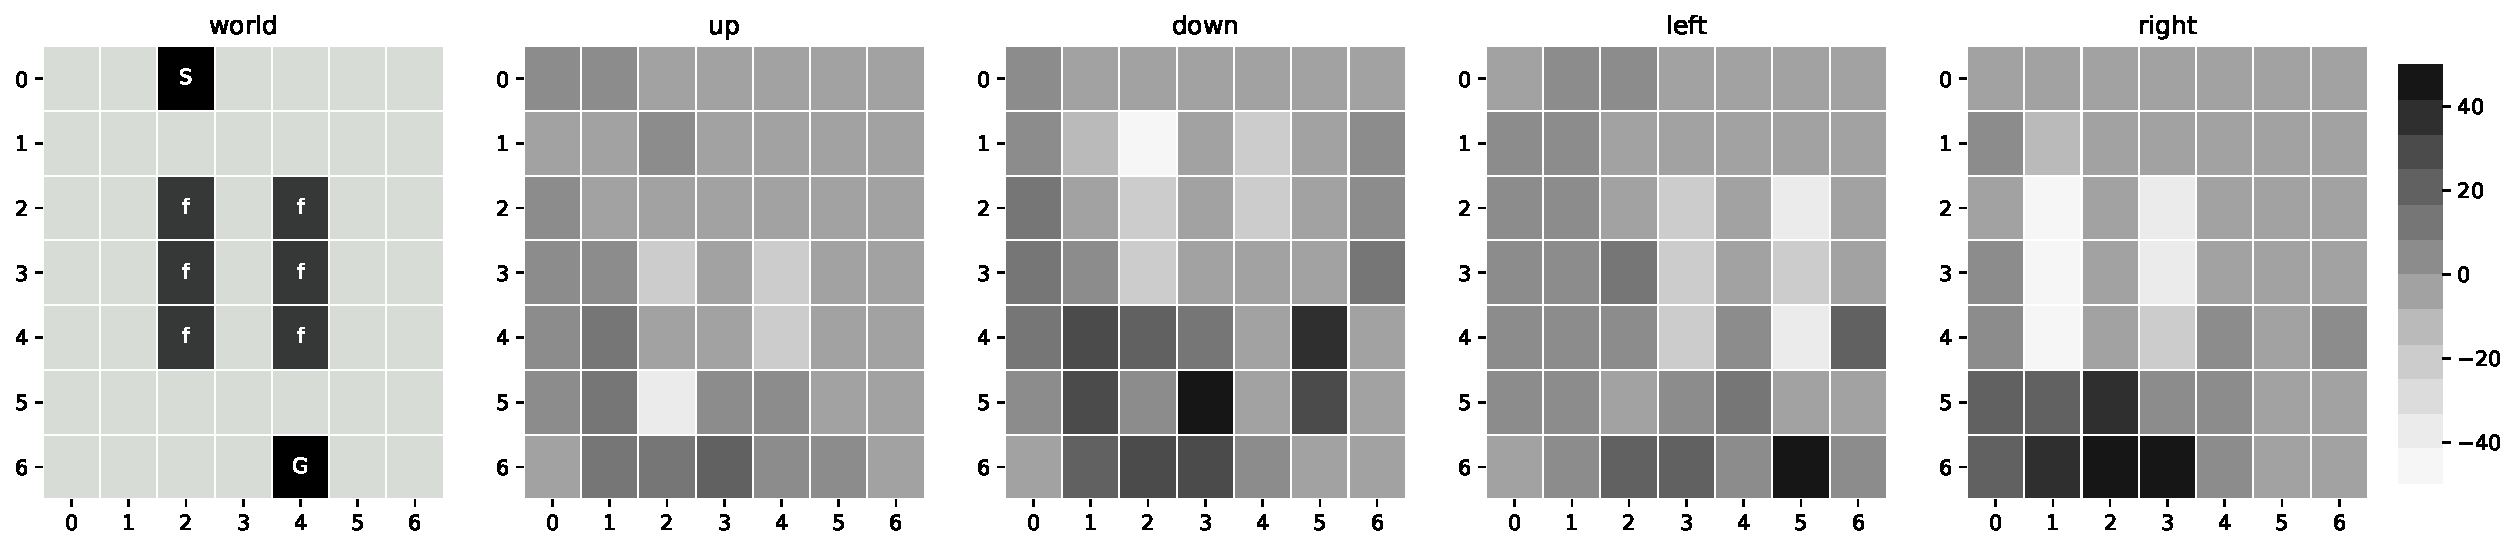
\includegraphics[width=\linewidth]{./images/fmlpda_figure_11_6_a.pdf}} \\
\end{tabular}
}
\end{center}
\caption[(a) A visualization of the final action-value table for an agent trained using SARSA on-policy temporal-difference learning across the grid world after $350$ episodes. (b) The cumulative reward earned from each episode.  (c) An illustration of the target policy learned by the agent after $350$ episodes. (d) The path the agent will take from the start state to the goal state when greedily following the target policy.]{(a) A visualization of the final action-value table for an agent trained using SARSA on-policy temporal-difference learning across the grid world after $350$ episodes. (b) The cumulative reward earned from each episode.  (c) An illustration of the target policy learned by the agent after $350$ episodes. The arrows show the direction with the highest entry in the action-value table for each state. (d) The path the agent will take from the start state to the goal state when greedily following the target policy.}

\label{fig:rl_grid_world_sarsa}
\end{figure}
\end{frame} 

 \begin{frame}
   \addtocounter{subfigure}{1}
\begin{figure}[!tbh]
\begin{center}
{\setlength{\tabcolsep}{0.05em}
\begin{tabular}{c}
	\subfigure[Cumulative Reward]{\label{fig:rl_grid_world_sarsa_returns}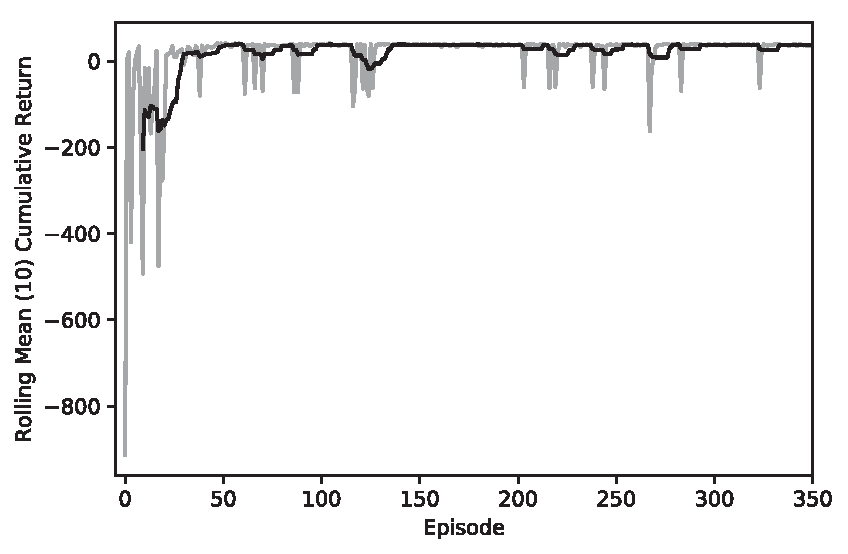
\includegraphics[width=0.42\linewidth]{./images/fmlpda_figure_11_6_b.pdf}}~\subfigure[Policy]{\label{fig:rl_grid_world_sarsa_policy}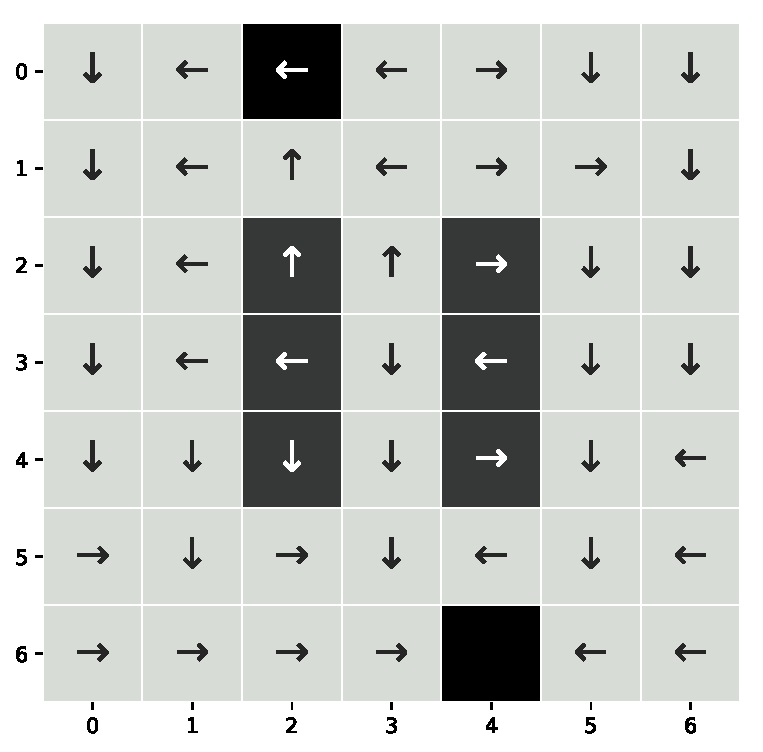
\includegraphics[width=0.27\linewidth]{./images/fmlpda_figure_11_6_c.pdf}}~\subfigure[Offline Path]{\label{fig:rl_grid_world_sarsa_offline_path}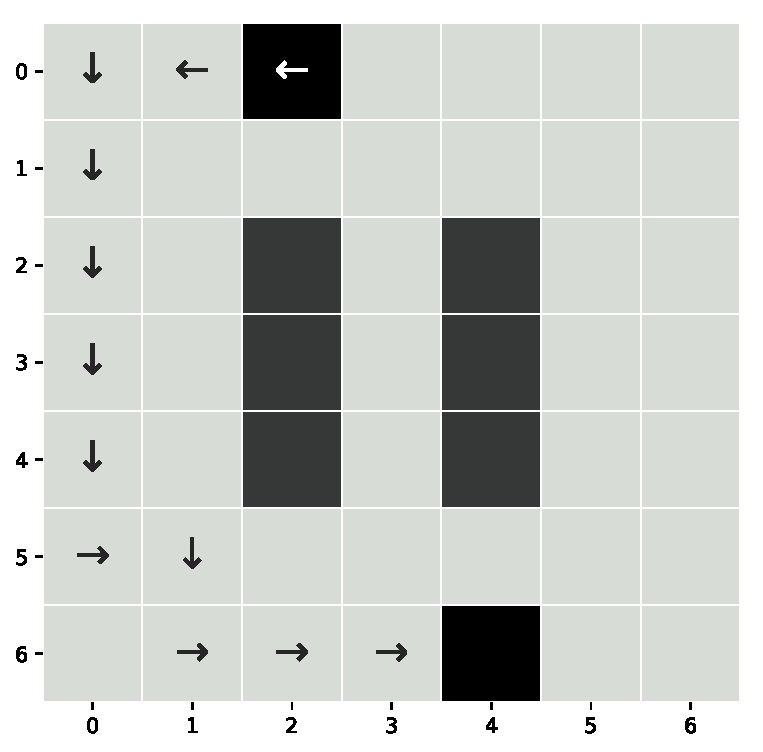
\includegraphics[width=0.27\linewidth]{./images/fmlpda_figure_11_6_d.pdf}}  \\	
\end{tabular}
}
\end{center}
\caption[(a) A visualization of the final action-value table for an agent trained using SARSA on-policy temporal-difference learning across the grid world after $350$ episodes. (b) The cumulative reward earned from each episode.  (c) An illustration of the target policy learned by the agent after $350$ episodes. (d) The path the agent will take from the start state to the goal state when greedily following the target policy.]{(a) A visualization of the final action-value table for an agent trained using SARSA on-policy temporal-difference learning across the grid world after $350$ episodes. (b) The cumulative reward earned from each episode.  (c) An illustration of the target policy learned by the agent after $350$ episodes. The arrows show the direction with the highest entry in the action-value table for each state. (d) The path the agent will take from the start state to the goal state when greedily following the target policy.}

\label{fig:rl_grid_world_sarsa}
\end{figure}
\end{frame} 


\subsection{Deep Q Networks}



 \begin{frame} 
\begin{figure}[tbh]
\begin{center}
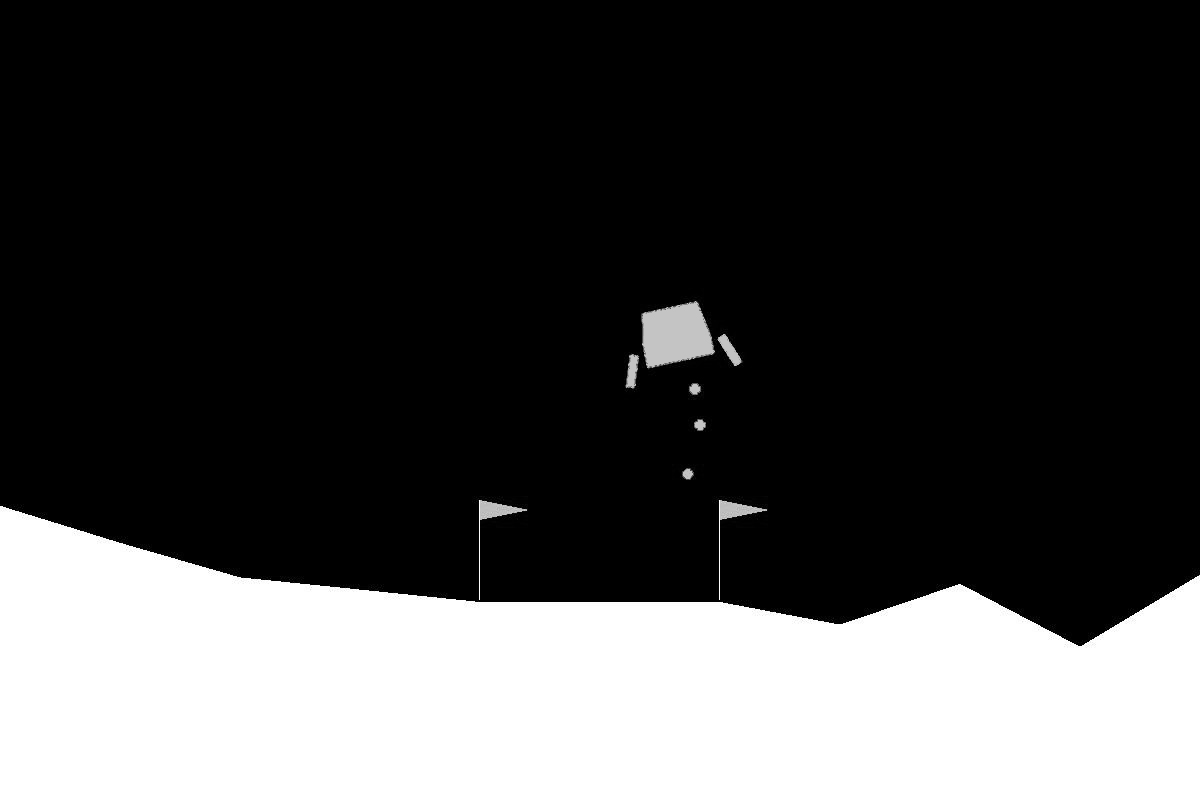
\includegraphics[width=0.55\textwidth]{./images/fmlpda_figure_11_7.jpg} 
\end{center}
\caption{The Lunar Lander environment. The aim of the game is to control the spaceship starting from the top of the world and attempting to land on the landing pad.}
\label{fig:rl_lunar_lander_env}
\end{figure}
\end{frame} 



 \begin{frame} 
\begin{figure}[tbh]
\begin{center}
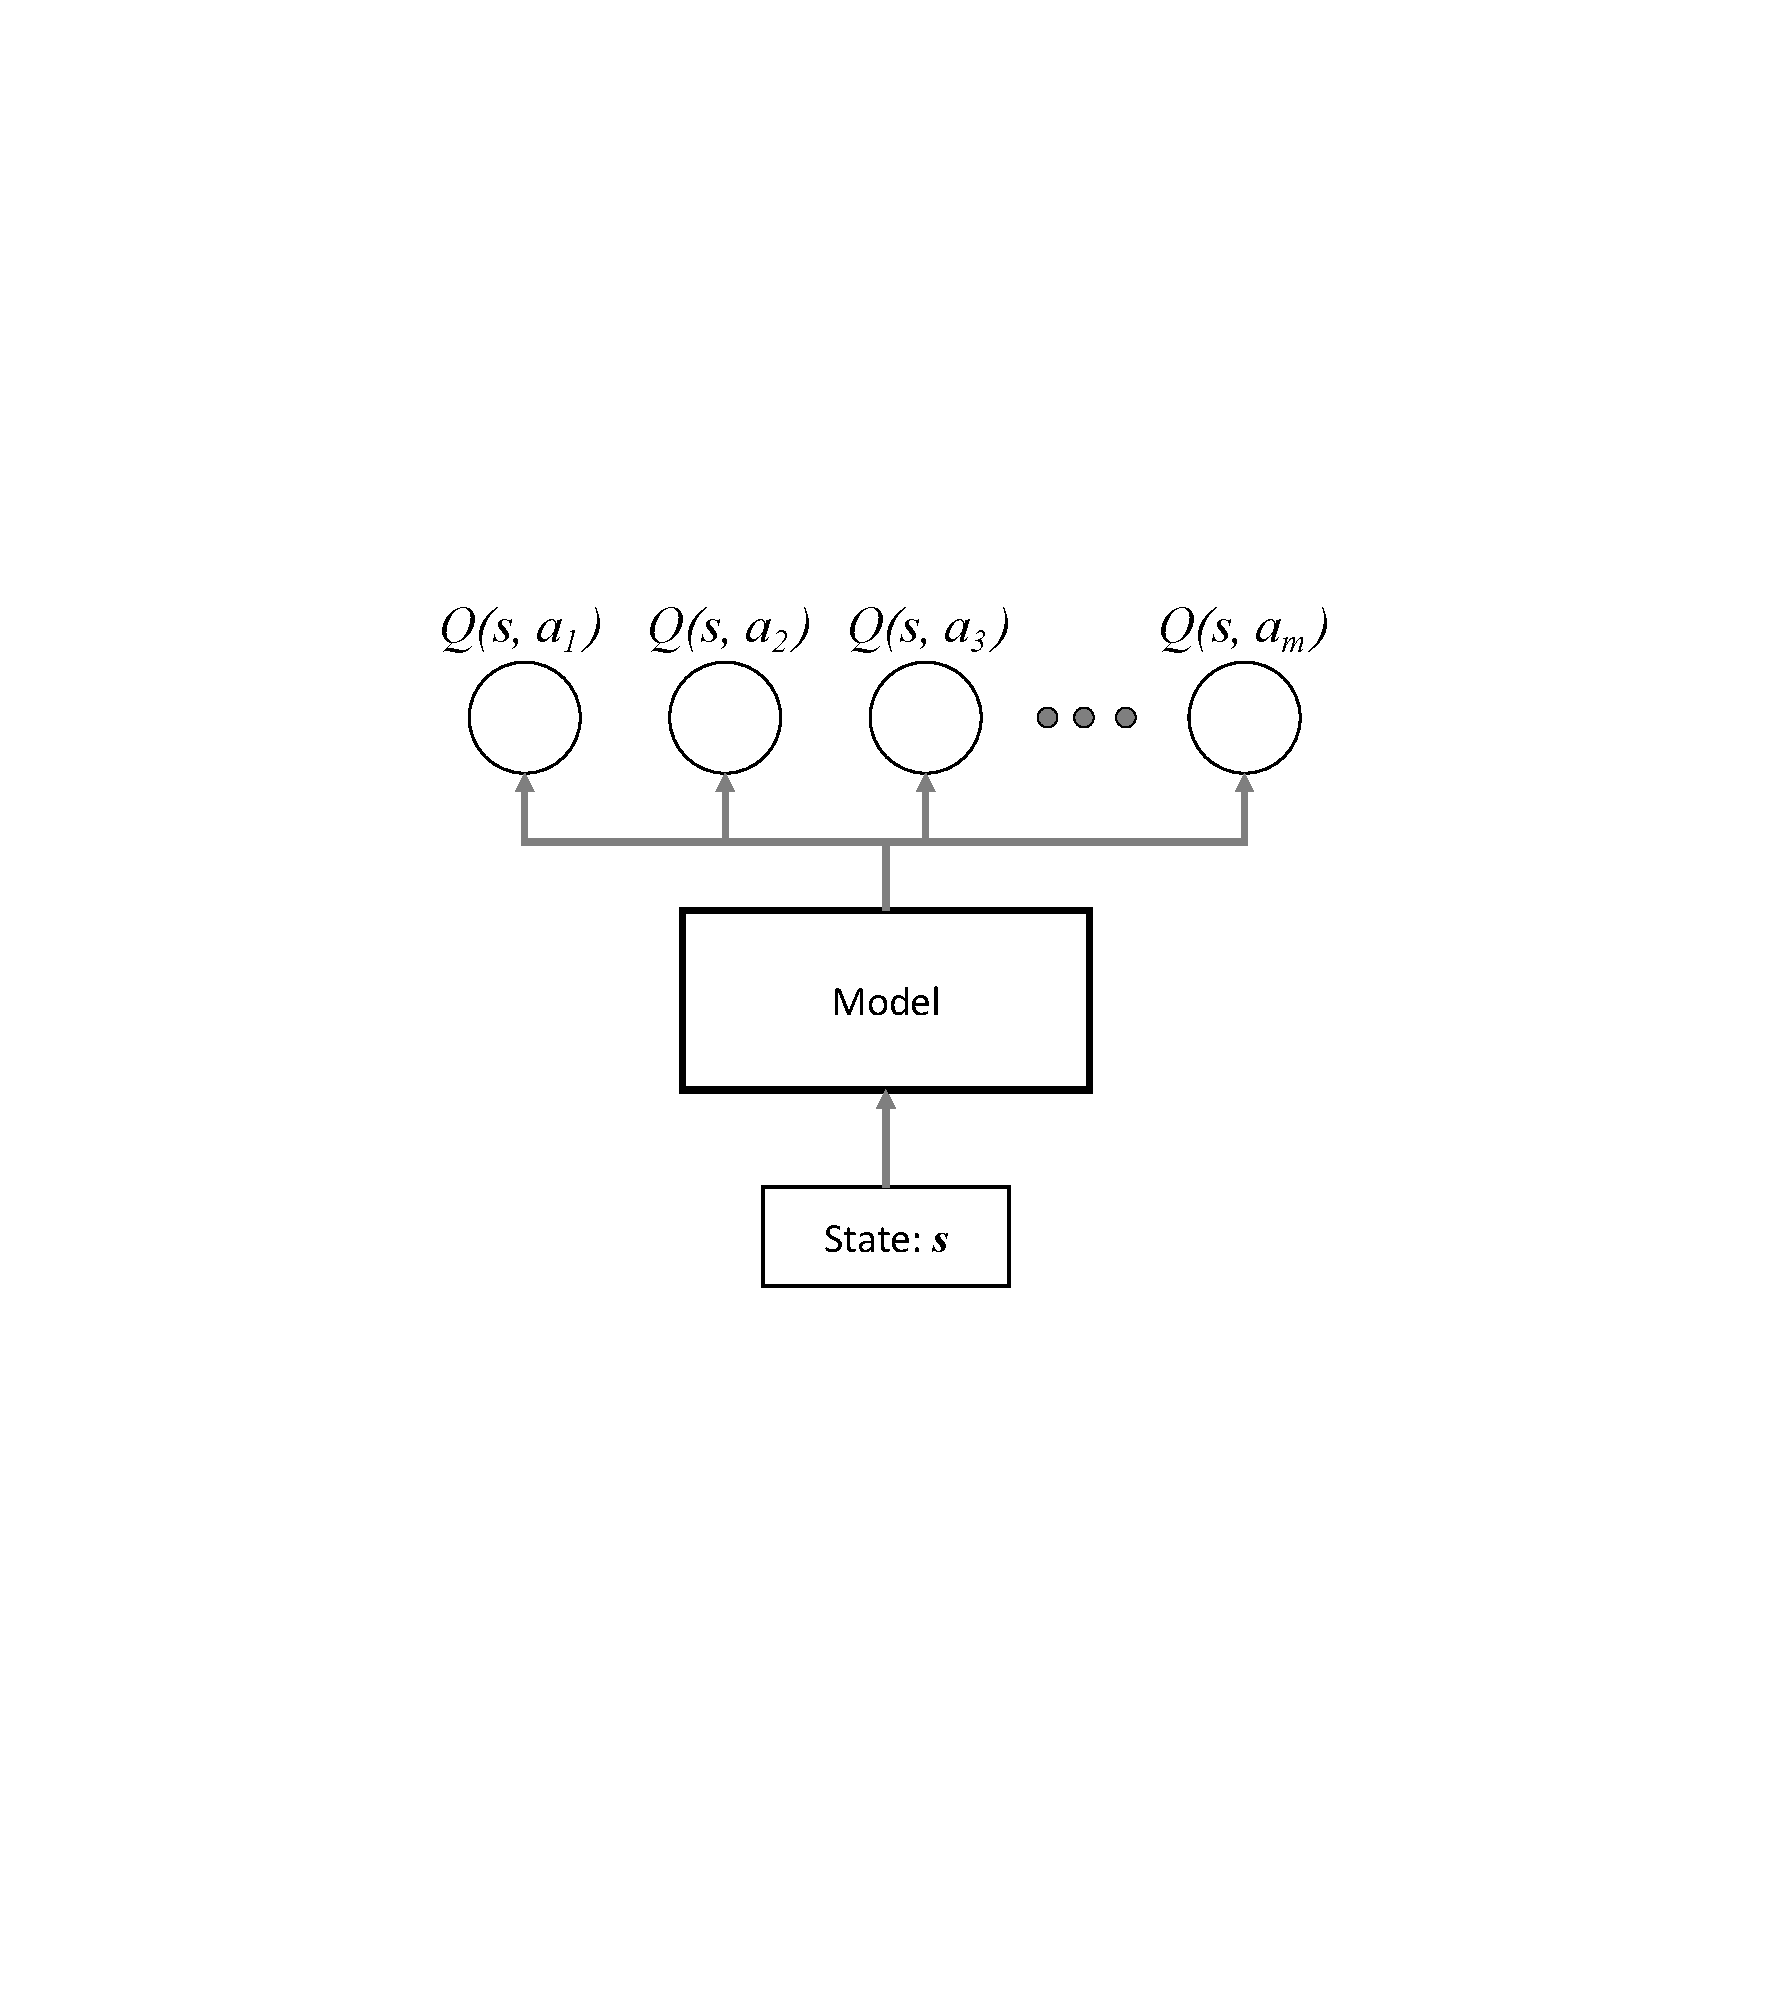
\includegraphics[width=0.5\textwidth]{./images/fmlpda_figure_11_8.pdf}
\end{center}
\caption{Framing the action-value function as a prediction problem.}
\label{fig:rl_dqn_architecture}
\end{figure}
\end{frame} 



 \begin{frame} 
\begin{equation}
\mathbb{M}(s_{t}, a_t) \thickapprox Q_{\pi}(s_t, a_t)
\end{equation}

~\\

\begin{equation}
\mathbb{M}(s_{t}) \thickapprox Q_{\pi}(s_t, a_t)
\end{equation}
\end{frame} 



 \begin{frame} 
 \begin{scriptsize}
\begin{alignat}{2}
\mathcal{L}(Q_{\mathbb{M}_{\mathbf{W}}}(s_t)) & = \left(t_i - Q_{\mathbb{M}_{\mathbf{W}}}\left(s_{t}, a_t\right)\right)^2 \\
~ & = \left(r_t +\gamma\max_{a_{t+1}}Q_{\mathbb{M}_{\mathbf{W}}}\left(s_{t+1}, a_{t+1}\right) - Q_{\mathbb{M}_{\mathbf{W}}}\left(s_{t}, a_t\right)\right)^2
\label{eqn:dqn_loss}
\end{alignat}
\end{scriptsize}

~\\

\begin{scriptsize}
\begin{alignat}{1}
\frac{\partial\mathcal{L}(Q_{\mathbb{M}_{\mathbf{W}}}(s_t, a_{t})) }{\partial \mathbf{W}} = \left(r_t +\gamma\max_{a_{t+1}}Q_{\mathbb{M}_{\mathbf{W}}}\left(s_{t+1}, a_{t+1}\right) - Q_{\mathbb{M}_{\mathbf{W}}}\left(s_{t}, a_t\right)\right)
\frac{\partial Q_{\mathbb{M}_{\mathbf{W}}}(s_t, a_t)}{\partial \mathbf{W}}
\label{eqn:dqn_loss_gradient}
\end{alignat}
\end{scriptsize}
\end{frame} 


\begin{frame}[plain]
\scriptsize{Pseudocode description of the \keyword{naive neural Q-learning} algorithm.}

%\begin{algorithm}[htb]
%\caption{Pseudocode description of the \keyword{naive neural Q-learning} algorithm.}
%\label{alg:naive_n_q_learning}
\begin{footnotesize}
\begin{algorithmic}[1]
\State initialize weights, $\mathbf{W}$,  in action-value function network, $Q_{\mathbb{M}}$, to random values
\For{each episode}
\State reset $s_{t}$ to the initial agent state
\Repeat
    \label{alg_ln:nnql_naive_choose_action}
    \State{select action, $a_{t}$, based on policy, $\pi$, the current state, $s_{t}$, and action-value network output, $Q_{\mathbb{M}}(s_{t}, a_{t})$ }
    \label{alg_ln:nnql_naive_take_action}
    \State take action $a_{t}$ and observing reward, $r_{t}$, and new state, $s_{t+1}$
     \label{alg_ln:nnql_generate_target}
    \State generate a target feature
    \begin{equation*}
     t = r_{t} +\gamma\max_{{a_{t+1}}}Q_{\mathbb{M}}\left(s_{t+1}, a_{t+1}\right)
    \end{equation*}
     \State{perform an iteration of stochastic gradient descent using a single training instance $<s_{t}, t>$}
\Until{agent reaches terminal state}
\EndFor
\end{algorithmic}
\end{footnotesize}
%\end{algorithm}
\end{frame} 



 \begin{frame}[plain]
\begin{figure}[!tbh]
\begin{center}
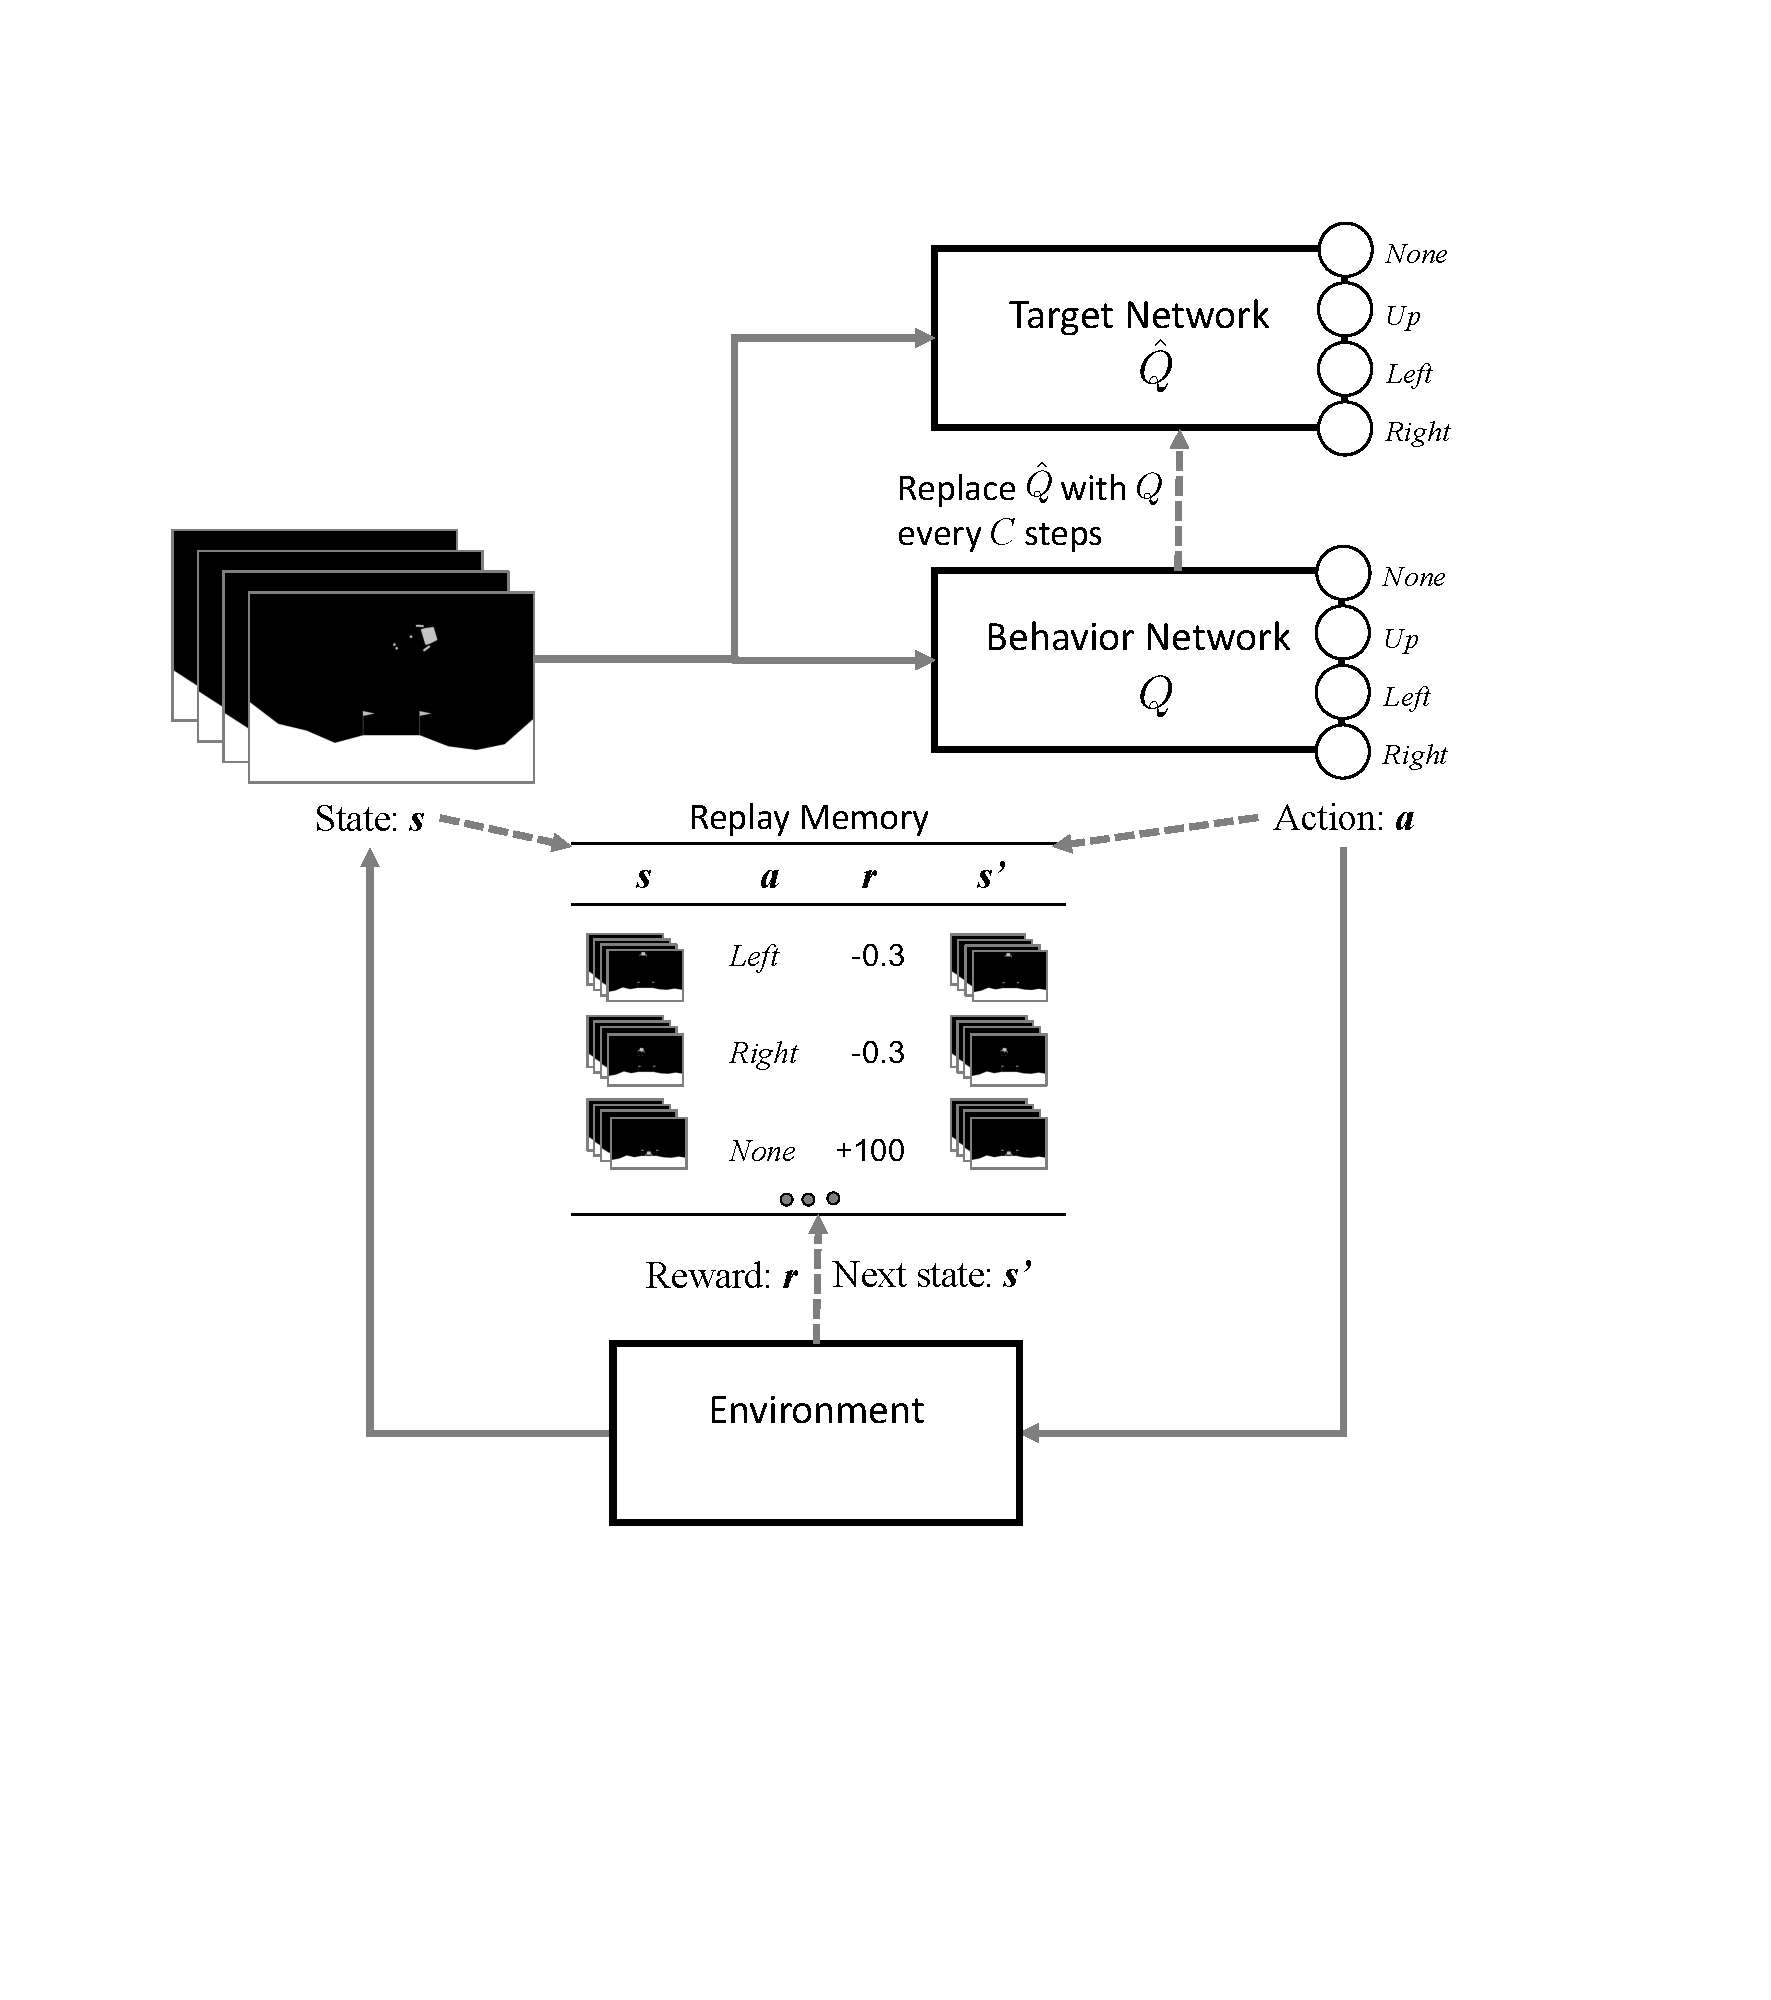
\includegraphics[width=0.7\textwidth]{./images/fmlpda_figure_11_9.pdf}
\end{center}
\caption{An illustration of the DQN algorithm including experience replay and target network freezing.}
\label{fig:rl_dqn_architecture_detailed}
\end{figure}
\end{frame} 






\begin{frame}[plain]
\scriptsize{Pseudocode description of the \keyword{deep Q network} (DQN) algorithm.}
%\begin{algorithm}[htb]
%\caption{Pseudocode description of the \keyword{deep Q network} (DQN) algorithm.}
%\label{alg:dqn}
\begin{footnotesize}
\begin{algorithmic}[1]
\State initialize replay memory $\mathcal{D}$ with $N$ steps based on random actions
\State initialize weights, $\mathbf{W}$  in behavior action-value function network, $Q_{\mathbb{M}}$, to random values
\State initialize weights, $\widehat{\mathbf{W}}$  in target action-value function network, $\widehat{Q_{\mathbb{M}}}$ to $\mathbf{W}$
\For{each episode}
\State reset $s_{t}$ to the initial agent state
\Repeat
    \label{alg_ln:nnql_choose_action}
    \State{select action, $a_{t}$, based on agent's policy, $\pi$, the current state, $s_{t}$, and behavior network output, $Q_{\mathbb{M}}(s_{t}, a_{t})$ }
    \label{alg_ln:nnql_take_action}
    \State take action $a_{t}$ and observe the resulting reward, $r_{t}$, and new state, $s_{t+1}$
    \State add tuple $\left<s=s_t, a=a_t, r=r_t, s'=s_{t+1}\right>$ as a new instance in $\mathcal{D}$
    \State randomly select a mini-batch of $b$ instances from $\mathcal{D}$ to give $\mathcal{D}_{b}$
    \State generate target feature values for each instance, $\left<s_i, a_i, r_i, s'_{i}\right>$ in $\mathcal{D}_{b}$ as: 
     \begin{equation*}
     t_i = r_i +\gamma\max_{a'}\widehat{Q_{\mathbb{M}}}\left(s'_{i}, a'\right)
     \end{equation*}
     \State perform an iteration of mini-batch gradient descent using $\mathcal{D}_{b}$
     \State every $C$ steps let $\widehat{Q_{\mathbb{M}}} = Q_{\mathbb{M}}$
\Until{agent reaches terminal state}
\EndFor
\end{algorithmic}
%\end{algorithm}
\end{footnotesize}
\end{frame} 


 \begin{frame}
\begin{figure}[!t]
\begin{center}
{\setlength{\tabcolsep}{0.05em}
\begin{tabular}{rr}  
	\multicolumn{2}{c}{\subfigure[Poor performance in the Lunar Lander environment early in the learning process.]{\label{fig:rl_lunar_lander_bad}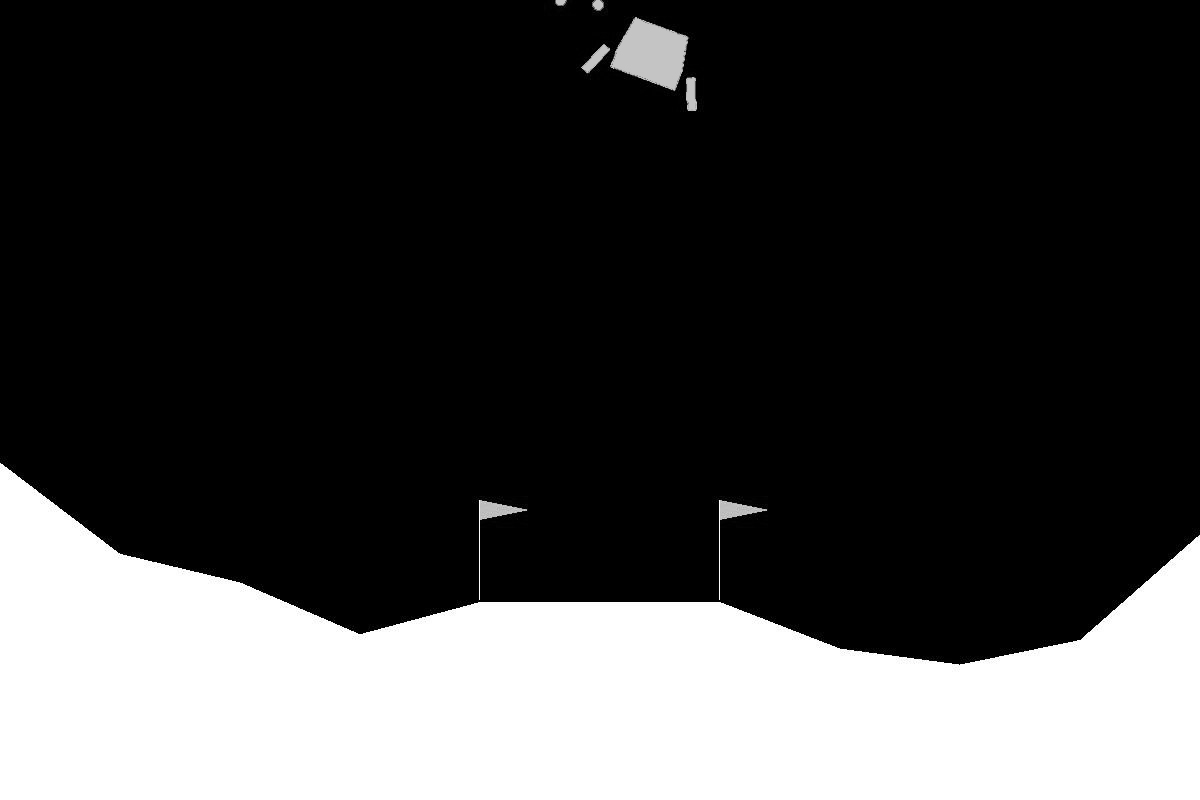
\includegraphics[width=0.24\linewidth]{./images/fmlpda_figure_11_10_a_i.jpg}~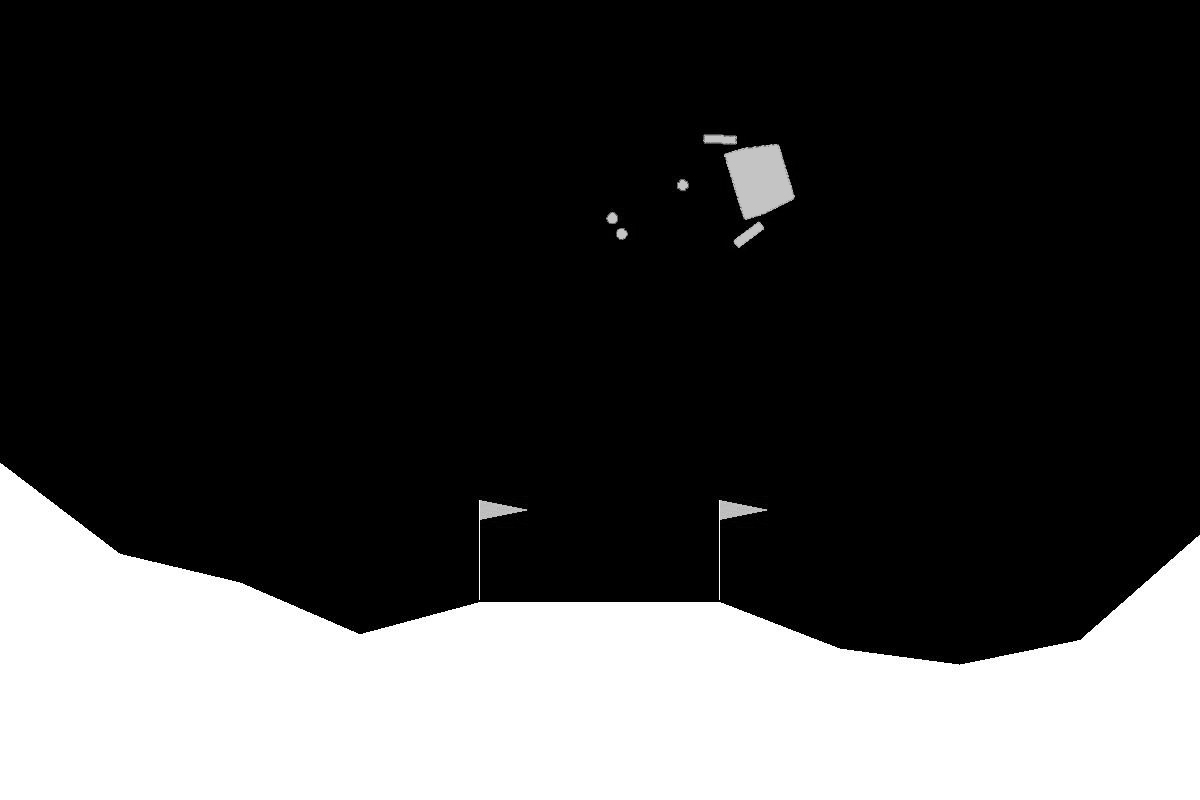
\includegraphics[width=0.24\linewidth]{./images/fmlpda_figure_11_10_a_ii.jpg}~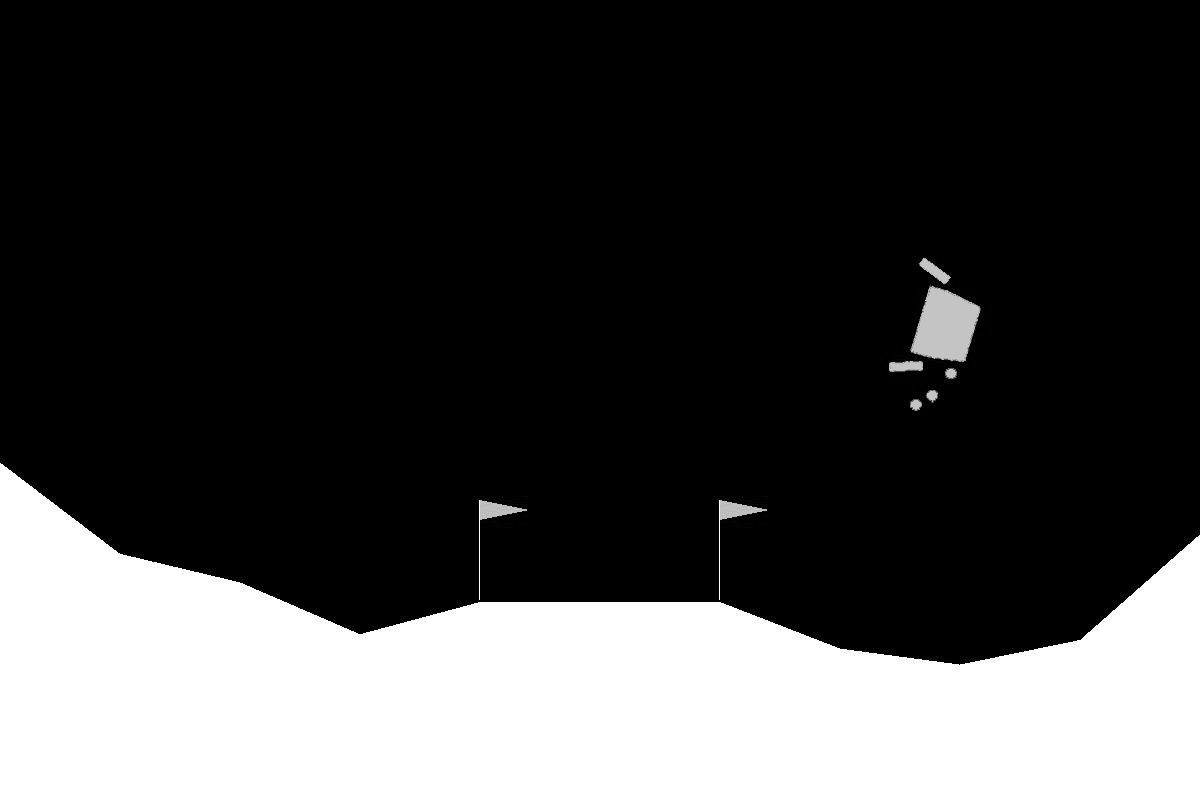
\includegraphics[width=0.24\linewidth]{./images/fmlpda_figure_11_10_a_iii.jpg}~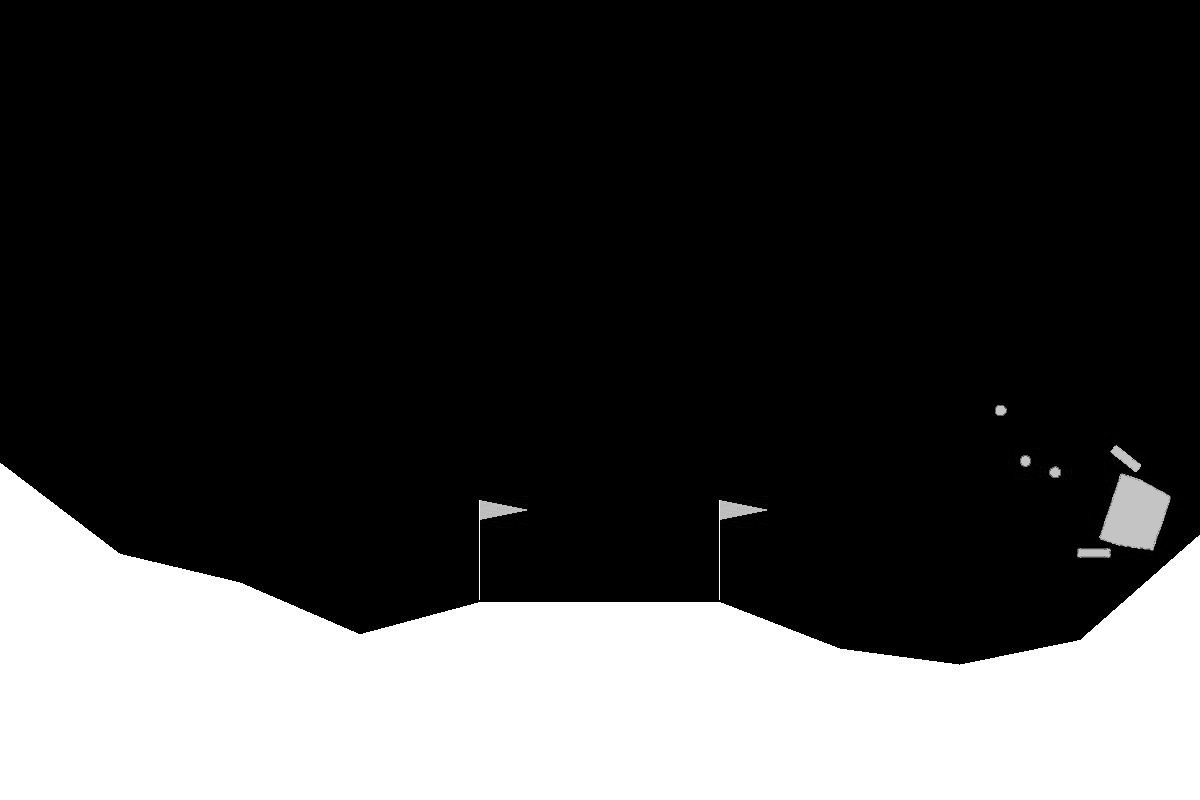
\includegraphics[width=0.24\linewidth]{./images/fmlpda_figure_11_10_a_iv.jpg}} } \\
\end{tabular}
}	
\end{center}
\caption{(a) Frames from an episode early in the training process in which the agent performs poorly. (b) Frames from an episode near the end of the learning process where the agent is starting to be very effective. (c) Changing episode returns during DQN training. The gray line shows a 50-episode moving average to better highlight the trend.}
\label{fig:rl_lunar_lander}
\end{figure}
\end{frame} 

 \begin{frame}
\addtocounter{subfigure}{1}
\begin{figure}[!t]
\begin{center}
{\setlength{\tabcolsep}{0.05em}
\begin{tabular}{rr}  
	\multicolumn{2}{c}{\subfigure[Good performance in the Lunar Lander environment after $30{,}000$ learning steps.]{\label{fig:rl_lunar_lander_good}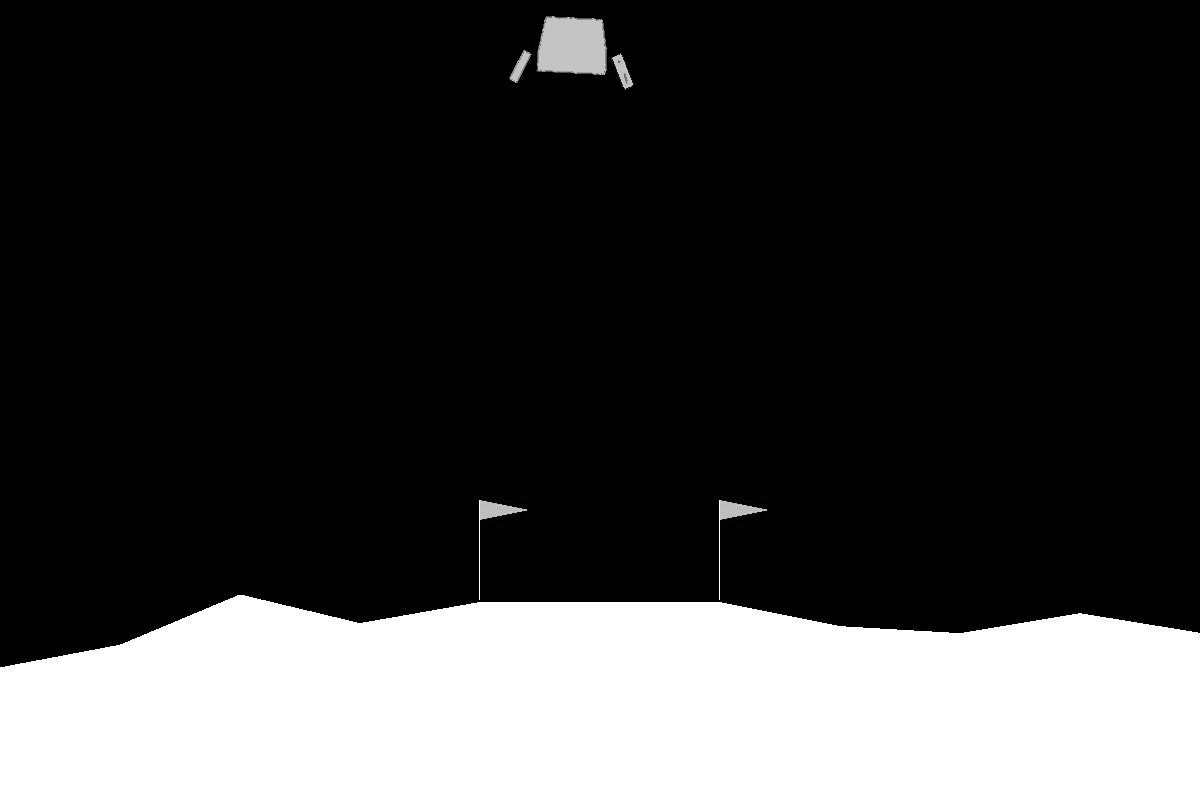
\includegraphics[width=0.24\linewidth]{./images/fmlpda_figure_11_10_b_i.jpg}~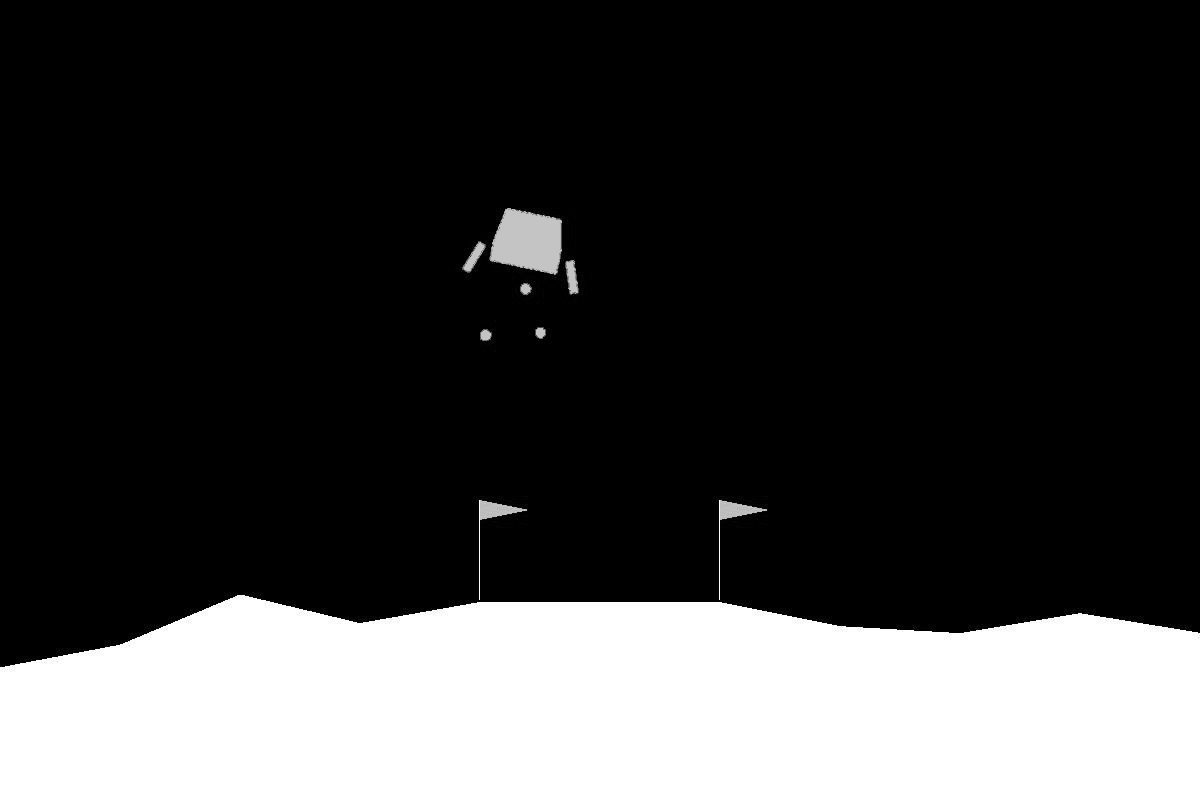
\includegraphics[width=0.24\linewidth]{./images/fmlpda_figure_11_10_b_ii.jpg}~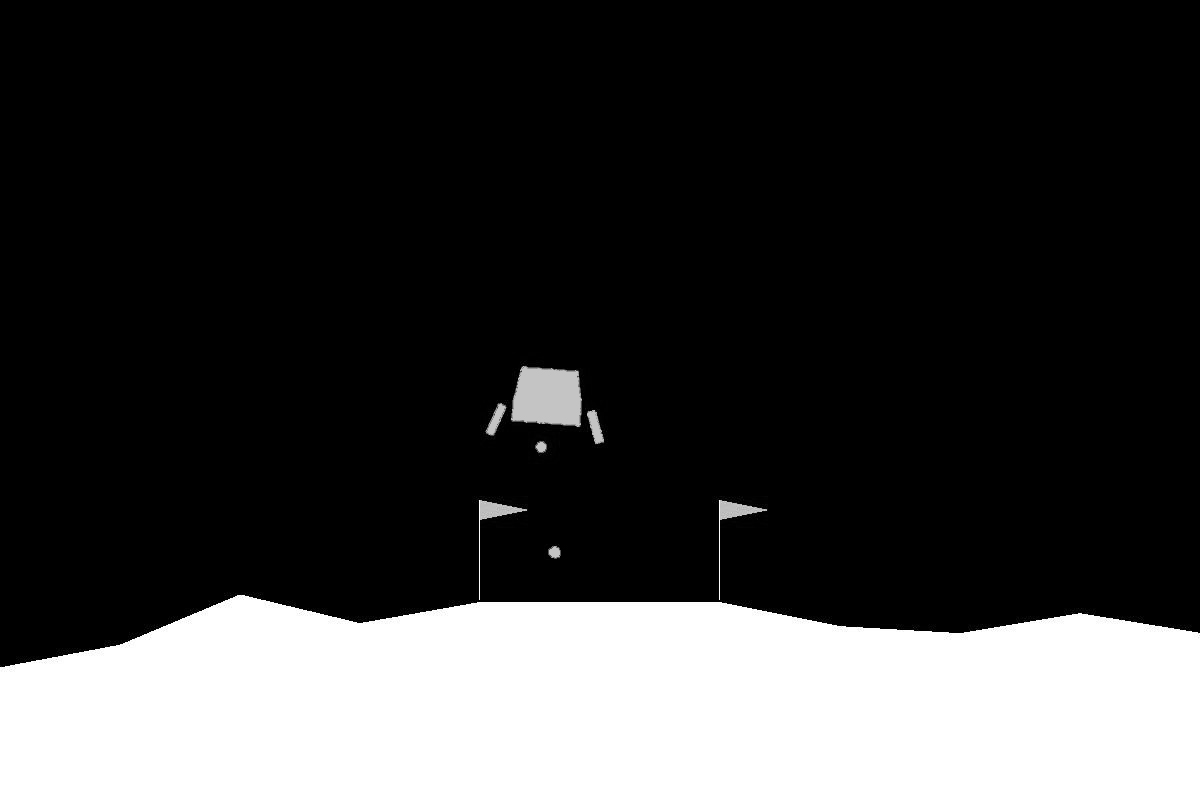
\includegraphics[width=0.24\linewidth]{./images/fmlpda_figure_11_10_b_iii.jpg}~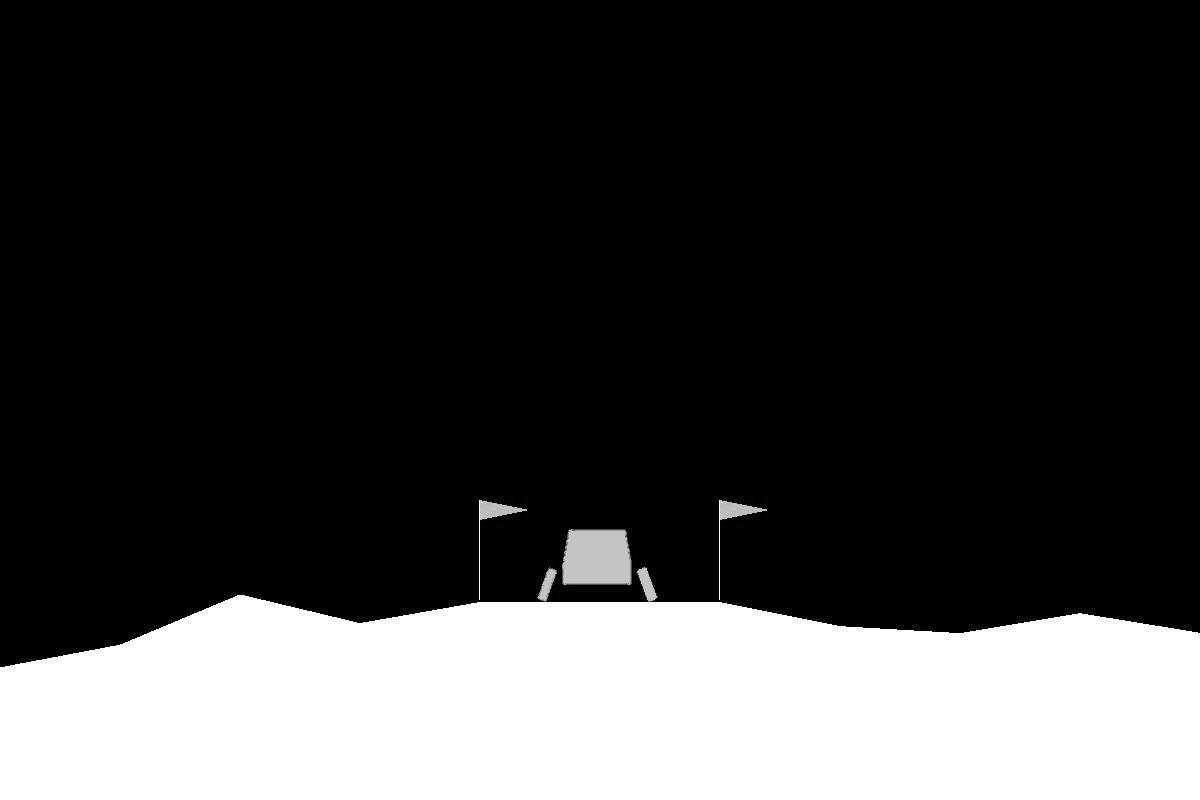
\includegraphics[width=0.24\linewidth]{./images/fmlpda_figure_11_10_b_iv.jpg}}} \\	
\end{tabular}
}	
\end{center}
\caption{(a) Frames from an episode early in the training process in which the agent performs poorly. (b) Frames from an episode near the end of the learning process where the agent is starting to be very effective. (c) Changing episode returns during DQN training. The gray line shows a 50-episode moving average to better highlight the trend.}
\label{fig:rl_lunar_lander}
\end{figure}
\end{frame} 


 \begin{frame}
\addtocounter{subfigure}{2}
\begin{figure}[!t]
\begin{center}
{\setlength{\tabcolsep}{0.05em}
\begin{tabular}{rr}  
	\multicolumn{2}{c}{\subfigure[Changing return during training.]{\label{fig:rl_lunar_lander_returns}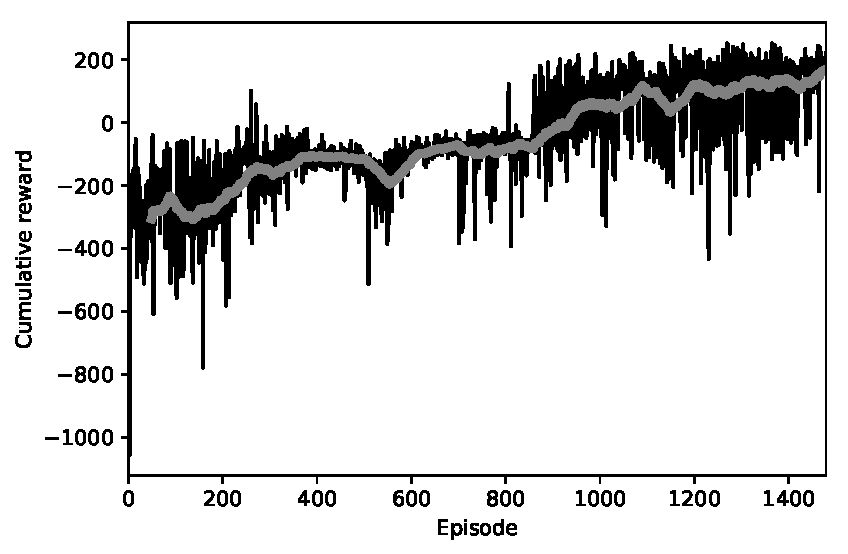
\includegraphics[width=0.48\linewidth]{./images/fmlpda_figure_11_10_c.pdf}}} \\
\end{tabular}
}	
\end{center}
\caption{(a) Frames from an episode early in the training process in which the agent performs poorly. (b) Frames from an episode near the end of the learning process where the agent is starting to be very effective. (c) Changing episode returns during DQN training. The gray line shows a 50-episode moving average to better highlight the trend.}
\label{fig:rl_lunar_lander}
\end{figure}
\end{frame} 



\SectionSlide{Summary}

\begin{frame}
\begin{itemize}
	\item In a reinforcement learning scenario an \keywordAlias{agent}{intelligent agent} inhabiting an \keyword{environment} attempts to achieve a \keyword{goal} by taking a sequence of \keywordAlias{actions}{action} to move it between \keywordAlias{states}{state}. 
	\item On completion of each action the agent receives an immediate scalar \keyword{reward} indicating whether the outcome of the action was positive or negative and to what degree. 
	\item To choose which action to take in a given state the agent uses a \keyword{policy}. 
	\item Policies rely on being able to assess the \keyword{expected return} of taking an action in a particular state, and an \keyword{action-value function} is used to calculate this. 

\end{itemize}
\end{frame}

\begin{frame}
\begin{itemize}
	\item The learning approaches described here are \keywordAlias{value-based}{value-based reinforcement learning} and \keywordAlias{model-free}{model-free reinforcement learning}. 
	\item \keywordAlias{Temporal-difference learning}{temporal-difference learning}, and its \keyword{Q-learning} (\keywordAlias{off-policy}{off-policy reinforcement learning}) and \keyword{SARSA} (\keywordAlias{on-policy}{on-policy reinforcement learning}) variants, is an important tabular methods for reinforcement learning. 
	\item \keywordAlias{Deep Q networks}{deep Q network} are an approximate approach to temporal difference learning based on deep neural networks.
\item One overarching point about reinforcement learning that is worth mentioning is that it comes at the cost of hugely increased computation. 
\end{itemize}
\end{frame}

\SectionSlide{Further Reading}

\begin{frame}
\begin{itemize}
	\item Key texts on intelligent agents: \citep{wooldridge1995intelligent,wooldridge2009introduction,macnamee2009agent}.  
	\item Key early foundation setting work: \citep{Howard:1960wa,Bellman:1957pc,Bellman:1957oy,Michie:ye,Michie:di}.  
	\item Sutton and Barto's textbook has remained the definitive work on reinforcement learning \citep{sutton2018reinforcement}.
	\item For a broader discussion on the challenges of defining reward functions: \citep{Asimov:1950zd,bostrom2003ethical}. 
	\item For more recent advances at the junction of reinforcement learning and deep learning: \citep{Sejnowski:2018yo,sutton2018reinforcement}.
\end{itemize}


\end{frame}

\begin{frame}
	%\tableofcontents
	 \tableofcontents[hideallsubsections]
\end{frame}

%\bibliographystyle{apalike}
\bibliographystyle{./mit-chicago-FMLPDA}
\bibliography{./FMLPDA2Bib_Brian}


\end{document}
